
\chapter{QUADRO METODOLÓGICO}

\par Foram apresentados os métodos adotados para realização de pesquisa,  tipo de pesquisa, contexto, participantes e outros.

\section{Tipo de Pesquisa}

\begin{comment}
  \par Pesquisa é ato de buscar e procurar pela resposta de algo. Marconi; Lakatos (2002, p. 15) definem pesquisa como “uma indagação minuciosa ou exame crítico e exaustivo na procura de fatos e princípios”.
\end{comment}
    
\par Existem diversos tipos de pesquisa, visando obter o verdadeiro objetivo foi utilizada a pesquisa aplicada, ou seja, foi desenvolvido um projeto de testes automatizados de \textit{software}, comprovando a eficiência em detectar erros e produzir um sistema de alta qualidade.

\par De acordo com \citeonline{aplicada}, "a pesquisa aplicada tem como motivação a necessidade de produzir conhecimento para aplicação de seus resultados, com o objetivo de contribuir para fins práticos, visando à solução mais ou menos imediata do problema encontrado na realidade”.

\par O projeto enquadrou-se no tipo de pesquisa aplicada, resolveu assim o problema específico, e foram criados vários tipos de testes automatizados, para comprovar que, no desenvolvimento, foi apontado o lugar no qual estava o erro no sistema.

\section{Contexto de Pesquisa}

\par Esta pesquisa será benéfica para os analistas de sistema e/ou desenvolvedores, pois através da implantação desses métodos será possível desenvolver um sistema de qualidade e sem erros.

\par O desenvolvedor tem como principais habilidades incluir o conhecimento dos fundamentos das linguagens de programação na qual trabalha, identificar erros e executar testes automatizados.
 
\par O analista de sistema sempre será o responsável por atuar nas análises e projetos de sistemas; levantamentos de requisitos e regras de negócio.

\par O teste automatizado auxilia o desenvolvimento de todos os envolvidos no projeto, o resultado deste envolvimento direto no desenvolvimento de um sistema com qualidade, auxilia na abrangência de minimizar a cobertura de erros.

\par O objetivo é desenvolver testes automatizados, visando detectar com precisão erros no sistema.


\section{Instrumentos}

\par Os requisitos e informações necessárias para o desenvolvimento do projeto foram obtidos através de questionário aplicado online e várias reuniões com os participantes do projeto.

\par O questionário foi uma forma de coletar informações através de perguntas bem elaboradas a um público específico. Segundo \citeonline{pesquisa}, questionário pode ser definido como um conjunto de perguntas que mede a opinião e interesse do respondente.

\par Foi aplicado no trabalho um questionário online, com oito perguntas, direcionadas para serem respondidas por pessoas que trabalham ou tem conhecimento na área de tecnologia da informação. As perguntas que foram feitas estão na apêndice desse trabalho.

\par As perguntas propostas tiveram por objetivo buscar informações sobre teste de \textit{software} automatizado, como uso do conhecimento e utilização por parte das empresas. A partir das repostas, obter dados direcionando qual tipo de teste automatizado é mais utilizado e quais as vantagens de usá-lo.

\par Com o resultado do questionário online que foi aplicado, pode-se concluir que 52,4\% utilizam teste unitários, 47,6\% teste de integração e 45,2\% teste funcional.

\par Foram feitas reuniões semanais entre os participantes do projeto para acompanhamento dos resultados das pesquisas em outras reuniões foram propostas várias melhorias.
    
\section{Procedimentos e Resultados}

\par Após os estudos das teorias em testes automatizados de \textit{softwares}, iniciou-se o período de desenvolvimento dos testes automatizados.

\subsection{Levantamento de Requisitos}

\par Quando foi feita a opção pela pesquisa, o objetivo era de entender como o uso de testes automatizados melhoram o processo de desenvolvimento do \textit{software} e a entrega final. As soluções geradas neste trabalho  atenderam os seguintes requisitos:

\begin{itemize}
\item Descrição e definição do funcionamento do teste automatizado;

\item Preparação do ambiente de desenvolvimento tanto da aplicação como dos testes que foram realizados com as ferramentas já citadas anteriormente;

\item Desenvolvimento de um aplicativo em html5, fazendo os testes de unidade, integração e funcional;

\item Desenvolvimento dos testes necessários realizados na aplicação desenvolvida;

\item Demonstração dos testes rodados em tempo real, e prevenção de qualquer falha no sistema, antes mesmo dele ser finalizado. 

\end{itemize}

\par Tendo estes paradigmas em mente, passou-se a desenvolver a aplicação \textit{web} de folha de pagamento, e assim mostrar como são feitos os testes automatizados e como acompanhar as seções seguintes.


\subsection{NodeJS}

\par Para o desenvolvimento do \textit{software} e o início dos testes automatizados, foi necessário a preparação do ambiente de desenvolvimento.

\par Na instalação do NodeJS é necessário acessar o site do NodeJS e baixar o arquivo "exe", e efetuar a instalação no padrão Windows,
através do \textit{link}:\url{https://nodejs.org/en/download/}. 


\begin{comment}
omo demonstrado nas figuras abaixo: 

\begin{figure}[!htb]
     \centering
     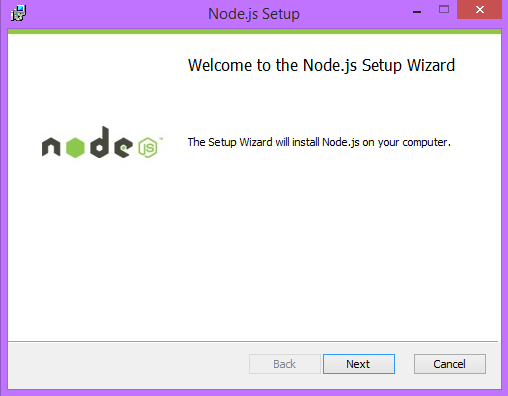
\includegraphics[width=10cm,height=15cm]{imagens/node1.png}
     \caption[NODEJS]{NODEJS.
     \textbf{Fonte: } Elaborado pelos autores.}
     \label{fig: nodejs}
\end{figure}

\begin{figure}[!htb]
     \centering
     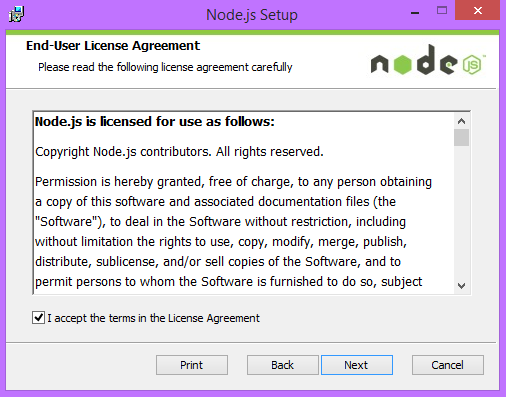
\includegraphics[width=10cm,height=8cm]{imagens/node2.png}
     \caption[NODEJS]{NODEJS.
     \textbf{Fonte: } Elaborado pelos autores.}
     \label{fig: nodejs}
\end{figure}

\begin{figure}[!htb]
     \centering
     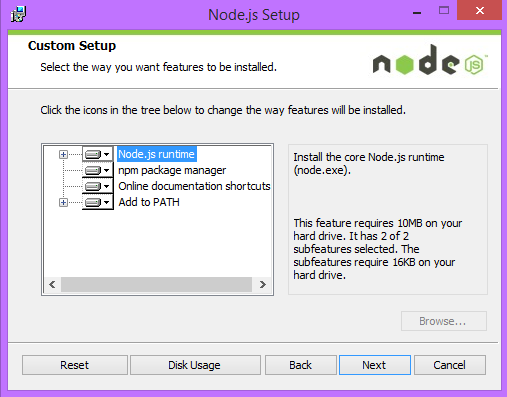
\includegraphics[width=10cm,height=9cm]{imagens/node3.png}
     \caption[NODEJS]{NODEJS.
     \textbf{Fonte: } Elaborado pelos autores.}
     \label{fig: nodejs}
\end{figure}

\begin{figure}[!htb]
     \centering
     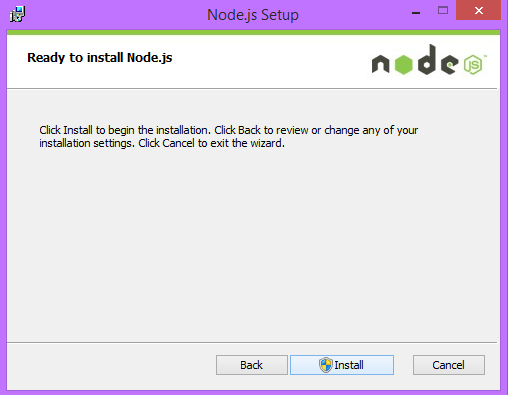
\includegraphics[width=10cm,height=8cm]{imagens/node4.png}
     \caption[NODEJS]{NODEJS.
     \textbf{Fonte: } Elaborado pelos autores.}
     \label{fig: nodejs}
\end{figure}

\begin{figure}[!htb]
     \centering
     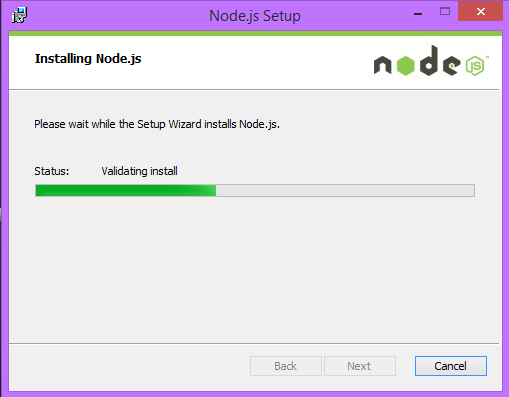
\includegraphics[width=10cm,height=8cm]{imagens/node5.png}
     \caption[NODEJS]{NODEJS.
     \textbf{Fonte: } Elaborado pelos autores.}
     \label{fig: nodejs}
\end{figure}

\begin{figure}[!htb]
     \centering
     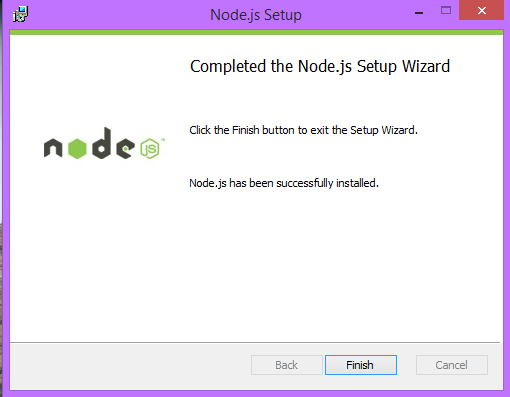
\includegraphics[width=10cm,height=8cm]{imagens/node6.png}
     \caption[NODEJS]{NODEJS.
     \textbf{Fonte: } Elaborado pelos autores.}
     \label{fig: nodejs}
\end{figure}
\end{comment}

%\clearpage
\newpage

\subsection{Instalação de dependências}


\par Para dar início ao desenvolvimento do projeto é necessário preparar o ambiente. Após ter instalado o \textit{NodeJS}, foi necessário instalar as dependências, utilizando o NPM \footnote{Node Package Manager}, para instalar as ferramentas que foram faladas no quadro teórico.

\par Abra o \textit{Prompt} de comando do S.O \footnote{Sistema Operacional} na pasta do projeto e digite \texttt{npm init}, conforme mostra Figura 1.


\begin{figure}[!htb]
    \caption[NPM init]{NPM init.
    
     \centering
     
     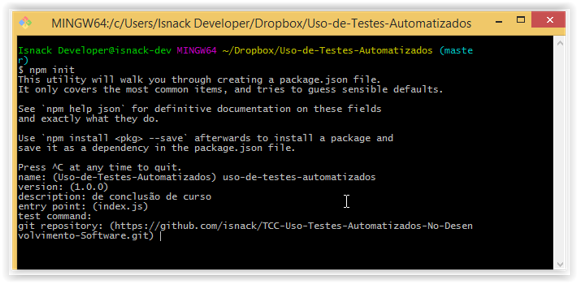
\includegraphics[width=12cm,height=10cm]{imagens/npm1.PNG}
     
     \textbf{Fonte: } Elaborado pelos autores.}
     \label{fig: npm init}
\end{figure}



\par É criado um arquivo \texttt{package.json}, este arquivo é responsável pelo gerenciamento das dependências do projeto e dos comandos dos testes que serão realizados posteriormente.

\par Abaixo a descrição dos campos que são requisitados para criação do arquivo \texttt{package.json}:

\begin{itemize}
 
 \item \texttt{Name}: Nome do Projeto.
 \item \texttt{Version}: Versão do Projeto.
 \item \texttt{Description}: Descrição do Projeto.
 \item \texttt{Entry Point}: Arquivo principal para inicializar o projeto.
 \item \texttt{Test Command}: Comando de testes. Nessa linha serão colocados comandos dos \textit{frameworks} que serão utilizados.
 \item \texttt{Git Repository}: Colocado o endereço do repositório do \textit{GitHub}.
 
\end{itemize}


\par Após os campos preenchidos é mostrado o esboço do arquivo que é gerado na pasta raiz do projeto, conforme mostra a Figura 2.

\begin{figure}[!htb]
    \caption[NPM ]{NPM.
    
     \centering
     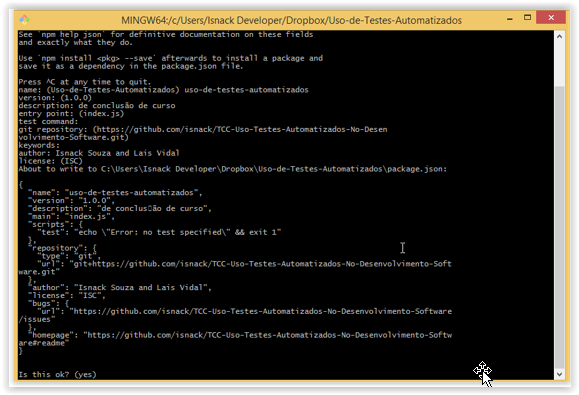
\includegraphics[width=12cm,height=10cm]{imagens/npm2.PNG}
     
     \textbf{Fonte: } Elaborado pelos autores.}
     \label{fig: npm}
\end{figure}


\par Após confirmar a criação, o arquivo é gerado na pasta do projeto, conforme mostra Figura 3.


\newpage
\begin{figure}[!htb]
    \caption[Arquivo Criado na Pasta ]{Arquivo Criado na Pasta.
     \centering
     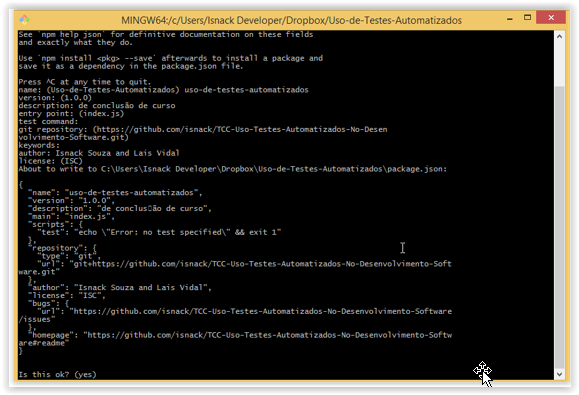
\includegraphics[width=12cm,height=8cm]{imagens/npm2.PNG}
     
     \textbf{Fonte: } Elaborado pelos autores.}
     \label{fig: Arquivo Criado na Pasta}
\end{figure}


\par Após inicializar o NPM é necessário executar os comandos de instalação dos pacotes das ferramentas \textit{CasperJS}, \textit{PhantomJS}, \textit{MochaJS} e \textit{ChaiJS}. Abaixo seguem os comandos que são executados:

\begin{itemize}
\item npm install casperjs -- save-dev
\item npm install phantomjs-prebuilt -- save-dev
\item npm install mocha chai  -- save-dev
\item npm install mongodb --save
\end{itemize}
\begin{figure}
  
  \caption[Exemplo de instalação das ferramentas ]{Exemplo de instalação das ferramentas.
     \centering
     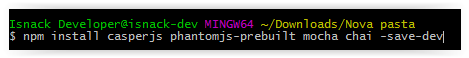
\includegraphics[scale=1]{imagens/npm4.PNG}
     
     \textbf{Fonte: } Elaborado pelos autores.}
     \label{fig: Exemplo de instalação das ferramentas}
\end{figure}



\newpage

\section{Testes}

\par Faz-se necessário a criação de uma pasta, nomeada \texttt{test}, para salvar os arquivos que são responsáveis pelos de testes, conforme mostra a Figura 5.

 \begin{figure}[!htb]
     \caption[Test ]{Test.
     \centering
     
     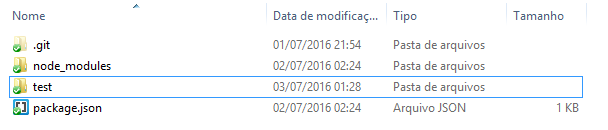
\includegraphics[scale=.75]{imagens/teste1.PNG}
     
     \textbf{Fonte: } Elaborado pelos autores.}
     \label{fig:test}
\end{figure}

\par Agora será criado um arquivo que executará os testes unitários, contendo o código fonte para cálculo do INSS.

\begin{comment}
 \begin{figure}[!htb]
     \caption[Teste Código Fonte ]{Teste Código Fonte.
     \centering
     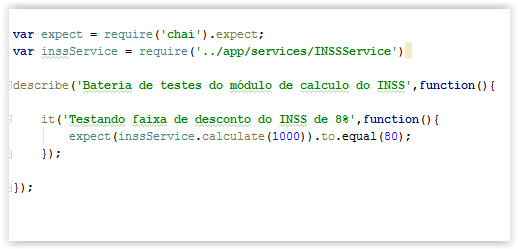
\includegraphics[width=12cm,height=8cm]{imagens/teste2.png}
     
     \textbf{Fonte: } Elaborado pelos autores.}
     \label{fig:teste código fonte}
\end{figure}
\end{comment}


\begin{lstlisting}[language=JavaScript, caption={[Teste de Código]{Teste de Código.  \textbf{Fonte:} Elaborado pelos autores.}}]
var expect = require('chai').expect;
var inssService = require('../app/services/INSSService')

describe('Bateria de teste do módulo de calculo do INSS',function(){
      it('Testando faixa de desconto do INSS de 8% ',function(){
        expect(inssService.calculate(1000).to.equal(80);
    });
});
\end{lstlisting}


\par A variável \texttt{expect} está recebendo os métodos do \textit{framework} \textit{Chai} que é responsável na execução dos testes, sua função é efetuar comparativo entre o valor de acordo com a regra especificada.

 \par A variável \texttt{inssService} recebe os serviços criados em arquivo, que é o módulo de cálculos. A função \texttt{describe}, descrita nas baterias de testes, e passada como parâmetro.
 
\par Foi necessário criar uma função padrão \texttt{it} na qual é feita uma descrição do teste a ser realizado (será testado a faixa de desconto de 8\%). Nessa função é utilizada a variável \texttt{expect} e o serviço \texttt{inssService} que é chamada de função \texttt{calculate} informando o salário bruto (1000), feito isso é chamado o método \texttt{.to.equal} informando o valor esperado (80). 

\par Definido o primeiro teste, roda-se o sistema para testar sua eficiência, e como não se tem os serviços implementados, é esperado mostrar um erro.

\par Ao executar os testes é necessário configurar um comando no arquivo \texttt{NPM} na linha de \textit{scripts}, basta adicionar o nome \texttt{test} passando o parâmetro \texttt{mocha}, conforme demonstra o Código 2.

\begin{comment}
 \begin{figure}[!htb]
     \caption[Configurar NPM - test ]{Configurar NPM - test.
     \centering
     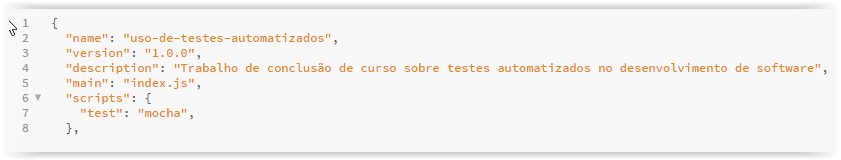
\includegraphics[width=12cm,height=8cm]{imagens/teste3.png}
    
     \textbf{Fonte: } Elaborado pelos autores.}
     \label{fig:configurar NPM - test}
\end{figure}
\end{comment}
 

\begin{lstlisting}[language=JavaScript, caption={[Configurar NPM test]{Configurar NPM test  \textbf{Fonte:} Elaborado pelos autores.}}]
{
"name": "uso-de-testes-automatizados",
"version": "1.0.0",
"description": "Trabalho de conclusão de curso sobre testes automatizados no desenvolvimento de software",
"main": "index.js",
"scripts": {
    "test": "mocha",
},
\end{lstlisting}



\par Após essa configuração abra o \textit{prompt} de comando dentro da pasta raiz do projeto, execute o comando \texttt{npm test} que executará o comando \textit{mocha}, conforme demonstra Figura 6.
 


\begin{figure}[!htb]
    \caption[NPM test ]{Npm test.
     \centering
     
     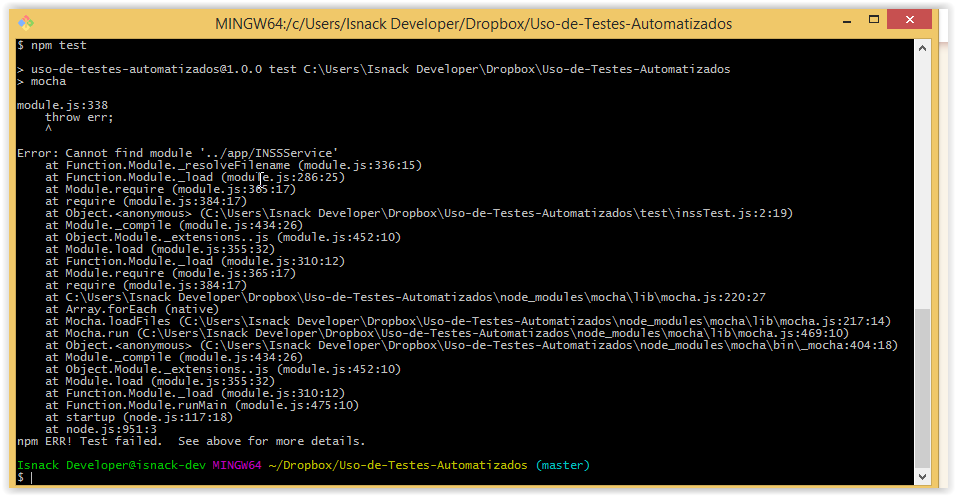
\includegraphics[scale=0.5]{imagens/teste4.png}
     
     \textbf{Fonte: } Elaborado pelos autores.}
     \label{fig:npm test}
\end{figure}

\newpage
\par O teste falhou porque não foi encontrado o módulo do INSS, para resolver isto, é necessário criar o módulo para o teste passar. Criado o módulo que foi salvo na pasta \texttt{services}, o método retornará o valor esperado e o objetivo é fazer o teste passar do jeito mais simples possível, a função retorna o valor 80, conforme mostra Código 3.

\begin{comment}
\begin{figure}[!htb]
     \caption[Modulo INSS ]{Modulo INSS.
     \centering
     
     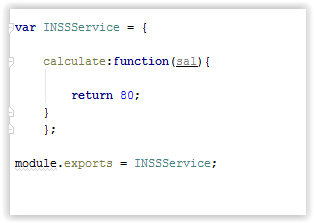
\includegraphics[width=12cm,height=8cm]{imagens/teste5.png}
    
     \textbf{Fonte: } Elaborado pelos autores.}
     \label{fig:modulo inss}
\end{figure}
\end{comment}


\begin{lstlisting}[language=JavaScript, caption={[Módulo INSS.]{Módulo INSS.  \textbf{Fonte:} Elaborado pelos autores.}}]
var INSSService = {

    calculate:function(sal){
       return 80;
   }
};
module.exports = INSSService;
\end{lstlisting}


\par Criado o serviço de cálculo com um retorno simples, roda-se o teste novamente para verificar se este erro passa.

\begin{figure}[!htb]
    \caption[Criação do primeiro teste INSS ]{Criação do primeiro teste INSS.
     \centering
     
     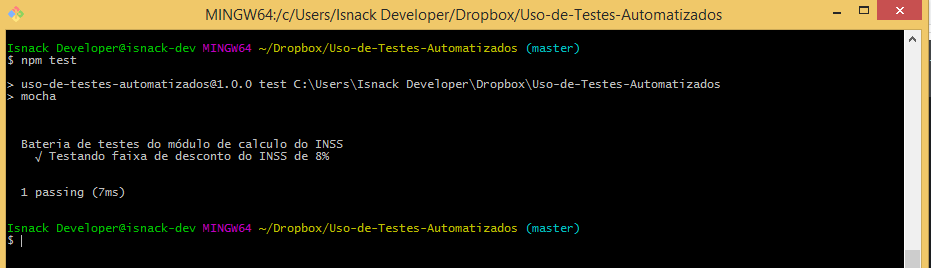
\includegraphics[scale=0.5]{imagens/teste6.png}
     
     \textbf{Fonte: } Elaborado pelos autores.}
     \label{fig:primeiro teste inss}
\end{figure}


\par Verifica-se que o teste passou conforme mostra Figura 7, após isso foram criados mais testes, conforme mostra Código 4, o objetivo é fazer os testes passarem, e assim, o código ser melhorado. Serão explicados todos os cenários que foram testados.

\begin{comment}
\begin{figure}[!htb]
    \caption[Criação de todos os testes INSS ]{Criação de todos os teste INSS.
     \centering
     
     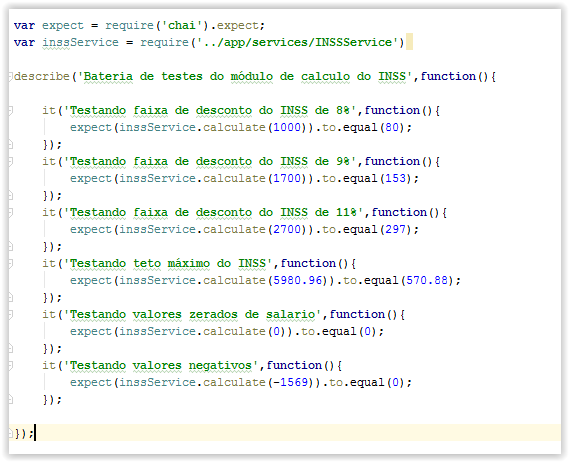
\includegraphics[width=12cm,height=8cm]{imagens/teste7.png}
     
     \textbf{Fonte: } Elaborado pelos autores.}
     \label{fig:todos teste inss}
\end{figure}
\end{comment}



\newpage

\begin{lstlisting}[language=JavaScript, caption={[Criação de todos os testes INSS.]{Criação de todos os testes INSS.  \textbf{Fonte:} Elaborado pelos autores.}}]
var expect = require('chai').expect;
var inssService = require('../app/services/INSSService');
describe('Bateria de testes do módulo de calculo do INSS',function(){    
    it('Testando faixa de desconto do INSS de 8%',function(){
        expect(inssService.calculate(1000)).to.equal(80);
    });
    it('Testando faixa de desconto do INSS de 9%',function(){
        expect(inssService.calculate(1700)).to.equal(153);
    });
    it('Testando faixa de desconto do INSS de 11%',function(){
        expect(inssService.calculate(2700)).to.equal(297);
    });
    it('Testando teto máximo do INSS',function(){
        expect(inssService.calculate(5980.96)).to.equal(570.88);
    });
    it('Testando valores zerados de salario',function(){
        expect(inssService.calculate(0)).to.equal(0);
    });
    it('Testando valores negativos',function(){
        expect(inssService.calculate(-1569)).to.equal(0);
    });
});

\end{lstlisting}

\par Os quatro primeiros cenários foram testadas as faixas de desconto do INSS de acordo com o MTPS – Ministério do Trabalho e Previdência Social, seguindo a tabela do ano vigente. 

\par Tabela para Empregado, Empregado Doméstico e Trabalhador Avulso.



\begin{figure}[!htb]
     \caption[Tabela INSS ]{Tabela INSS.
     \centering
     
     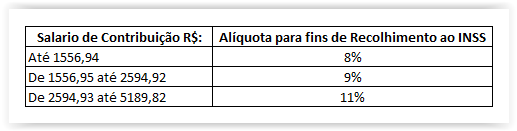
\includegraphics[width=8.89cm,height=2.75cm]{imagens/inss.png}
    
     \textbf{Fonte: } Elaborado pelos autores.}
     \label{fig:tabela inss}
\end{figure}




\par Nos últimos cenários foram testados valores com zero e negativo, deve retornar 0 para efeitos de cálculo. No Código 5 é mostrado o código do serviço pronto e os testes passando.

\begin{comment}

\begin{figure}[!htb]
     \caption[INSS Service ]{INSS Service.
     
     \centering
     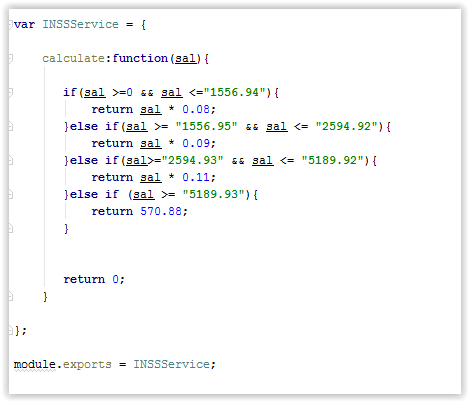
\includegraphics[width=12cm,height=8cm]{imagens/teste8.png}
    
     \textbf{Fonte: } Elaborado pelos autores.}
     \label{fig:INSS Service}
\end{figure}

\end{comment}

\newpage
\begin{lstlisting}[language=JavaScript, caption={[INSS Service.]{INSS Service.  \textbf{Fonte:} Elaborado pelos autores.}}]
var INSSService = {
        calculate:function(sal){
           if(sal >=0 && sal <="1556.94"){
              return sal * 0.08;
           }else if(sal >= "1556.95" && sal <= "2594.92"){
               return sal * 0.09;
           }else if(sal>="2594.93" && sal <= "5189.92"){
               return sal * 0.11;
           }else if (sal >= "5189.93"){
               return 570.88;
       }
         return 0;
    }
};
module.exports = INSSService;

\end{lstlisting}


\par Todos os testes que foram criados para o INSS, com suas respectivas faixas salariais, seus descontos e com valor negativo e zerado, mostrando que os testes passaram em todos os requisitos, conforme mostra a Figura 9.

\begin{figure}[!htb]
    \caption[Testes INSS Passando ]{Testes INSS Passando.
     \centering
     
     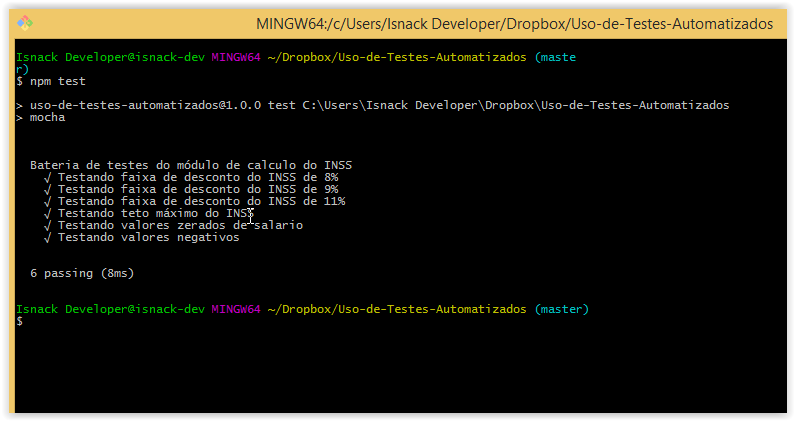
\includegraphics[scale=0.5]{imagens/teste9.png}
     
     \textbf{Fonte: } Elaborado pelos autores.}
     \label{fig:testes inss passando}
\end{figure}


\par Criado um arquivo que executará os testes unitários, que contém o código fonte para calculo do IR.
 
\begin{comment}
 \begin{figure}[!htb]
    \caption[Testes IR  ]{Testes IR.
     \centering
     
     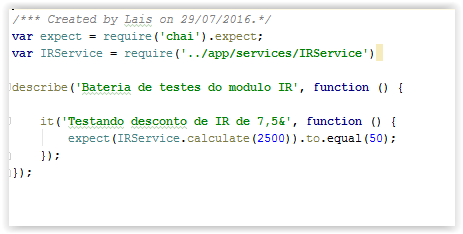
\includegraphics[width=12cm,height=8cm]{imagens/teste17.png}
     
     \textbf{Fonte: } Elaborado pelos autores.}
     \label{fig:testes ir}
\end{figure}
\end{comment}

\newpage

\begin{lstlisting}[language=JavaScript, caption={[IR Service.]{IR Service.  \textbf{Fonte:} Elaborado pelos autores.}}]
var expect = require('chai').expect;
var IRService = require('../app/services/IRService');

describe('Bateria de testes do Módulo IR',function(){
       it('Testando desconto de IR de 7,5%',function(){
       expect(IRService.calculate(2500)).to.equal(50);
    });
});

\end{lstlisting}



\par Abra o \textit{prompt} de comando, digite o comando \texttt{npm test}, o teste não irá passar, pois o valor esperado não é o correto, conforme mostra a Figura 10.

 \begin{figure}[!htb]
    \caption[Teste IR dando erro ]{Teste IR dando erro.
     \centering
     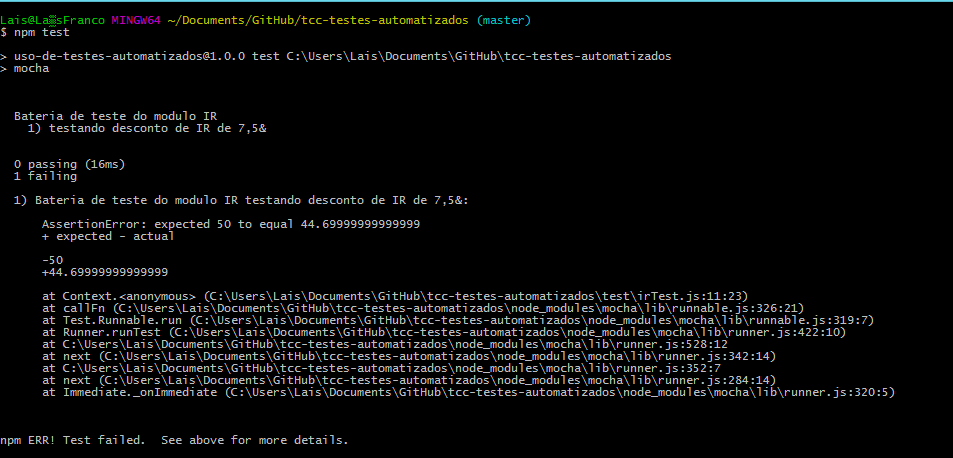
\includegraphics[scale=0.5]{imagens/teste16.png}
     
     \textbf{Fonte: } Elaborado pelos autores.}
     \label{fig:teste ir dando erro}
\end{figure}


\par Atualizando o valor esperando pela variável \texttt{to.equal}.



\begin{lstlisting}[language=JavaScript, caption={[Teste IR.]{Teste IR.  \textbf{Fonte:} Elaborado pelos autores.}}]
var expect = require('chai').expect;
var IRService = require('../app/services/IRServices');

describe('Bateria de teste do módulo IR', function(){
        it('Testando desconto de IR de 7,5%', funciton(){
        expect(IRService.calculate(2500)).to.equal(44,699999999999);
    });
});

\end{lstlisting}
\begin{comment}


 \begin{figure}[!htb]
     \caption[Teste Ir dando erro ]{Teste IR dando erro.
     \centering
     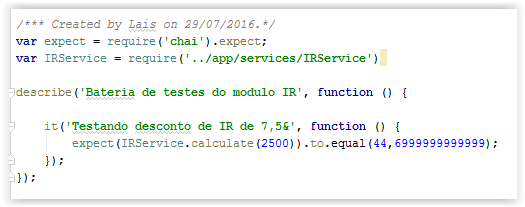
\includegraphics[width=12cm,height=6cm]{imagens/teste10.png}
    
     \textbf{Fonte: } Elaborado pelos autores.}
     \label{fig:teste ir dando erro}
\end{figure}
\end{comment}
\newpage

\par Após o valor atualizado o teste irá passar, conforme mostra a Figura 11.

\begin{figure}[!htb]
     \caption[NPM test - IR ]{NPM test - IR.
     \centering
     \raggedleft
     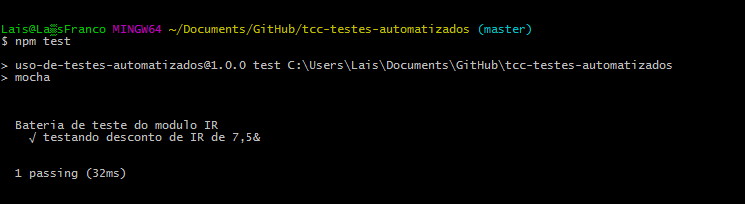
\includegraphics[scale=.70]{imagens/teste11.png}
    \centering
     \textbf{Fonte: } Elaborado pelos autores.}
     \label{fig:npm test - ir}
\end{figure}


\par Os quatro primeiros cenários foram testadas as faixas de desconto do IR de acordo com a tabela do ano vigente.


\begin{lstlisting}[language=JavaScript, caption={[Criação de todos os testes IR.]{Criação de todos os testes IR.  \textbf{Fonte:} Elaborado pelos autores.}}]
var expect = require('chai').expect;
var IRService = require('../app/services/IRService');
describe('Bateria de testes do modulo IR', function () {
         it('Testando desconto de IR de 7,5%', function () {
          expect(IRService.calculate(2500)).to.be.closeTo(44.70,0.01);
      });
         it('Testando desconto de IR de 15%', function () {
            expect(IRService.calculate(3500)).to.equal(170.20);
     });
        it('Testando desconto de IR de 22,5%', function () {
         expect(IRService.calculate(4500)).to.equal(376.37);
     });
         it('Testando desconto de IR de 27,5%', function () {
          expect(IRService.calculate(5500)).to.be.closeTo(643.14,0.01);
     });
         it('Testando valor de IR negativo', function () {
          expect(IRService.calculate(-1979)).to.equal(0);
     });
         it('Testando valores zerados', function () {
          expect(0).to.equal(IRService.calculate(0));
     });
});

\end{lstlisting}
\begin{comment}


 \begin{figure}[!htb]
    \caption[Criação de todos os testes IR ]{Criação de todos os testes IR.
     \centering
     
     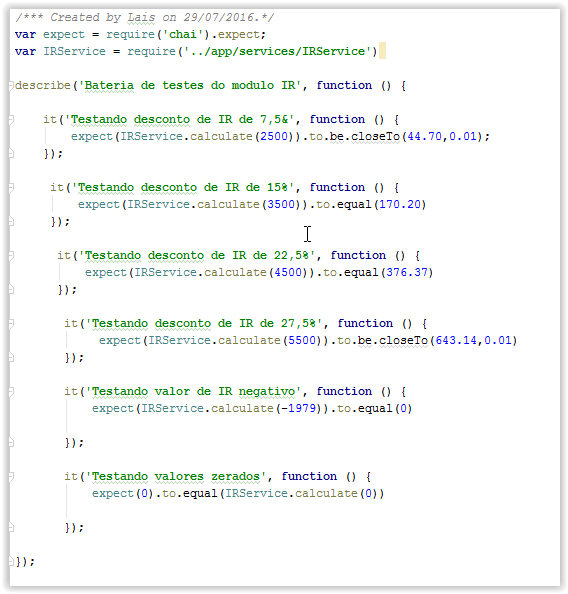
\includegraphics[width=12cm,height=10cm]{imagens/teste13.png}
     
     \textbf{Fonte: } Elaborado pelos autores.}
     \label{fig:criação de todos os testes INSS}
\end{figure}
\end{comment}

\newpage
\par  Foi utilizado nesse teste a função de comparação de resultados \texttt{to.be.closeTo}, nessa função é informado o valor que se deseja comparar com um intervalo de tolerância no resultado, que no caso é de 0.01.

\par Tabela de desconto do Imposto de Renda retido na fonte.

 \begin{figure}[!htb]
    \caption[Tabela IR ]{Tabela IR.
     \centering
     
     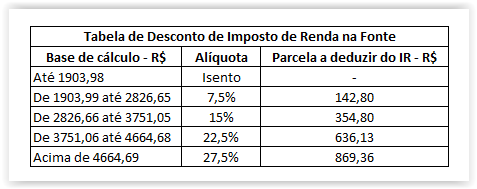
\includegraphics[width=12cm,height=6cm]{imagens/IR.png}
     
     \textbf{Fonte: } Elaborado pelos autores.}
     \label{fig:tabela ir}
\end{figure}

\par Os últimos cenários foram testados valores com zero e negativo, deve retornar 0 para efeitos de cálculo. No Código 9 é mostrado o código do serviço pronto e os testes passando.

\begin{comment}


\begin{figure}[!htb]
    \caption[IrService ]{IrService.
     \centering
     
     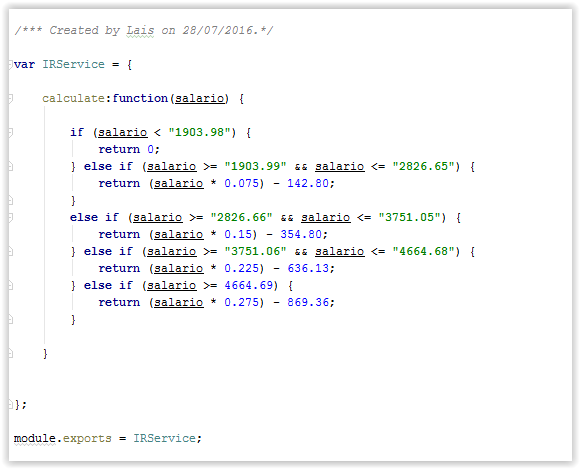
\includegraphics[width=12cm,height=6cm]{imagens/teste50.PNG}
     
     \textbf{Fonte: } Elaborado pelos autores.}
     \label{fig:modulo irService}
\end{figure}
\end{comment}


\begin{lstlisting}[language=JavaScript, caption={[IR Service.]{IR Service.  \textbf{Fonte:} Elaborado pelos autores.}}]
var IRService = {
    calculate:function(salario) {
        if (salario < "1903.98") {
            return 0;
        } else if (salario >= "1903.99" && salario <= "2826.65") {
            return (salario * 0.075) - 142.80;
        }
        else if (salario >= "2826.66" && salario <= "3751.05") {
            return (salario * 0.15) - 354.80;
        } else if (salario >= "3751.06" && salario <= "4664.68") {
            return (salario * 0.225) - 636.13;
        } else if (salario >= 4664.69) {
            return (salario * 0.275) - 869.36;
        }}
};
module.exports = IRService;

\end{lstlisting}

\newpage
\par Todos os testes que foram criados para o IR, com suas respectivas faixas salariais, seus descontos e com valor negativo e zerado, mostrando que os testes passaram em todos os requisitos, conforme mostra a Figura 13.

\begin{figure}[!htb]
    \caption[Teste de Ir Passando ]{Teste de Ir Passando.
     \centering
     
     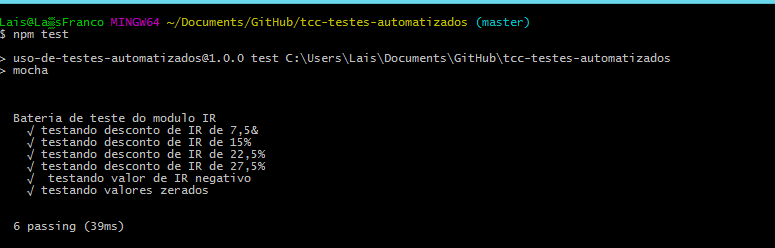
\includegraphics[width=12cm,height=8cm]{imagens/teste15.png}
     
     \textbf{Fonte: } Elaborado pelos autores.}
     \label{fig:teste de IR passando}
\end{figure}

 \par Criado os módulos de cálculo do desconto do INSS e do Imposto de Renda e devidamente testados, fez-se necessário a criação do módulo que calcula o salário líquido. Mas primeiro deve-se criar os testes.
\par Foi criado um arquivo nomeado \texttt{intergrationTestInssIr} dentro da pasta \texttt{test}, que é responsável pela realização dos testes de integração (INSS e IR), conforme mostra a Figura 14, a criação desse arquivo.
 
 
 \begin{figure}[!htb]
    \caption[Criação do arquivo para teste de integração ]{Criação do arquivo para teste de integração.
     \centering
     
     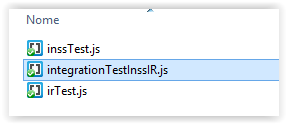
\includegraphics[scale=1.5]{imagens/teste18.png}
     
     \textbf{Fonte: } Elaborado pelos autores.}
     \label{fig:criação do arquivo para teste de integração}
\end{figure}

 \newpage
 \par O primeiro teste visa verificar um valor que possua desconto do INSS e não seja possível realizar o desconto do Imposto de renda (sendo o salário bruto 1500, o resultado esperado com o desconto de INSS é de 1380), conforme mostra Código 10.
 


 \begin{lstlisting} [language=JavaScript, caption={[ Primeiro teste de integração.]{ Primeiro teste de integração. \textbf{Fonte:} Elaborado pelos autores.}}]
var expect = require('chai').expect;
var IRService = require('../app/services/SalarioLiquidoService');
describe('Testa se os descontos de cada serviço está como especificado',function () {
            
   it('Salario faixa minima na qual é descontado somente o INSS', function () {
     expect(salarioLiquidoService.calculate(1500)).to.equal(1380);
    });         
});

\end{lstlisting}

\begin{comment}
 \begin{figure}[!htb]
     \caption[Primeiro teste de integração ]{Primeiro teste de integração.
     \centering
     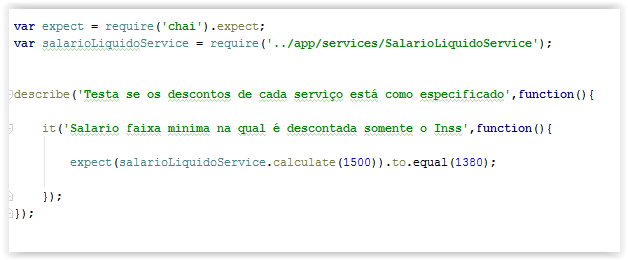
\includegraphics[width=12cm,height=6cm]{imagens/teste19.png}
    
     \textbf{Fonte: } Elaborado pelos autores.}
     \label{fig:primeiro teste de integração}
\end{figure}
\end{comment}


\par Executado o teste, verificou-se que, conforme o esperado, o teste falhou, pois não foi criado o serviço chamado \texttt{salarioLiquidoService}, conforme mostra Figura 15.

\begin{figure}[!htb]
    \caption[Teste falhando ]{Teste falhando.
     \centering
     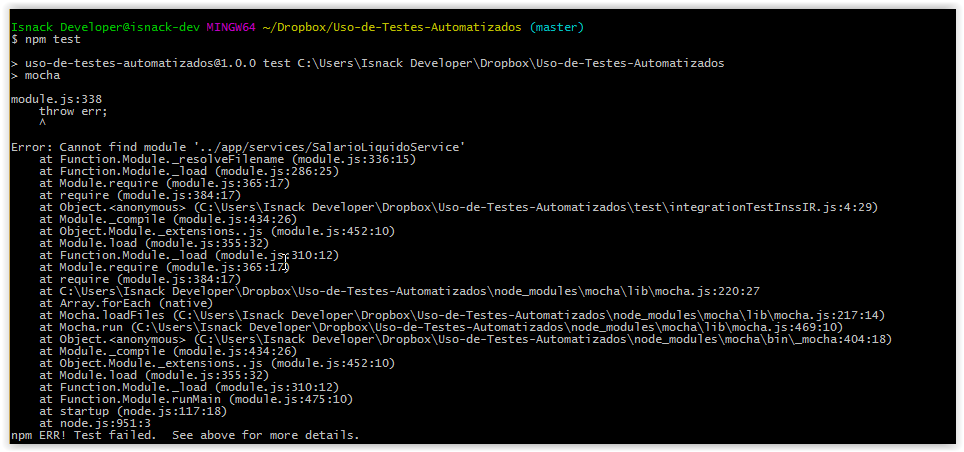
\includegraphics[scale=0.5]{imagens/teste20.png}
     
     \textbf{Fonte: } Elaborado pelos autores.}
     \label{fig:teste falhando}
\end{figure}


\par Após realizar o primeiro teste, foi criado o módulo para calcular o salário liquido dentro da pasta \texttt{services}, seguindo a mesma metodologia dos testes anteriores de criar uma solução simples e depois refatorar, ou seja, melhorar o código. O Código 11 faz essa demonstração.

\newpage


 
\begin{lstlisting}[language=JavaScript, caption={[Módulo de salário líquido.]{Módulo de salário líquido. \textbf{Fonte:} Elaborado pelos autores.}}]
var  IRService = require('./IRService');
var INSSService = require('./INSSService');

var SalarioLiquidoService = {
  calculate:function (salario) {

    var salarioBruto = salario;
    var valorDescontadoInss,salarioComDescontoInss,
        valorDescontadoIR,salarioLiquido;
    
    valorDescontadoInss = INSSService.calculate(salarioBruto);
    salarioComDescontoInss = salarioBruto - valorDescontadoInss;
    valorDescontadoIR = IRService.calculate(salarioComDescontoInss);
    salarioLiquido = salarioComDescontoInss - valorDescontadoIR;

   return salarioLiquido;
}};
module.exports =  SalarioLiquidoService;
\end{lstlisting}

\begin{comment}
\begin{figure}[!htb]
     \caption[Código do módulo de salário liquido ]{Código do módulo de salário liquido.
     \centering
     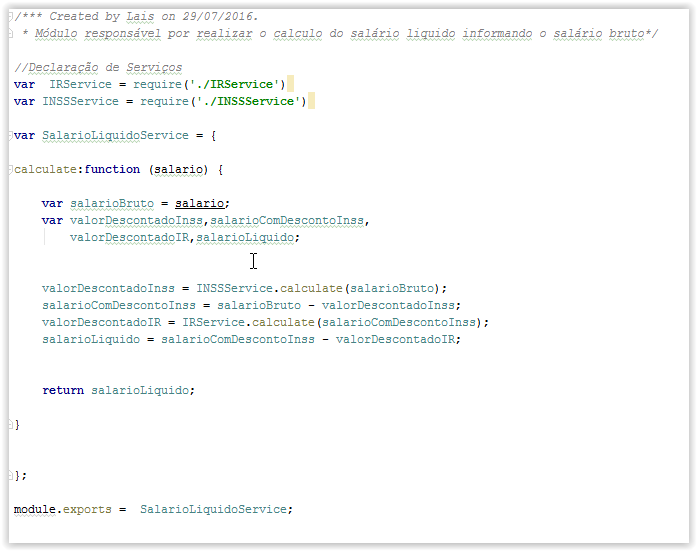
\includegraphics[width=12cm,height=6cm]{imagens/teste21.png}
     
     \textbf{Fonte: } Elaborado pelos autores.}
     \label{fig:código do módulo de salário liquido}
\end{figure}
\end{comment}

\par O módulo recebe o valor do salário bruto como parâmetro, em seguida é atribuído a variável, é chamada de \texttt{salarioBruto}, são criadas outras variáveis: \texttt{valorDescontadoInss}, \texttt{salarioComDescontoInss}, \texttt{valorDescontadoIR} e \texttt{salarioLiquido}.

\par A variável \texttt{valorDescontadoINSS} recebe como resultado o módulo de cálculo do desconto do INSS, e a variável \texttt{salarioComDescontoINSS} recebe o valor de  cálculo do salário bruto menos o desconto do INSS, \texttt{valorDescontadoIR} recebe como resultado o módulo de cálculo do Imposto de Renda e o \texttt{salarioLiquido} recebe o resultado final do salário menos os descontos de INSS e Imposto de Renda.

\par O teste foi executado novamente, conforme mostra a Figura 16.
\newpage
\begin{figure}[!htb]
      \caption[Teste de integração sendo rodado novamente ]{Teste de integração sendo rodado novamente.
     \centering
     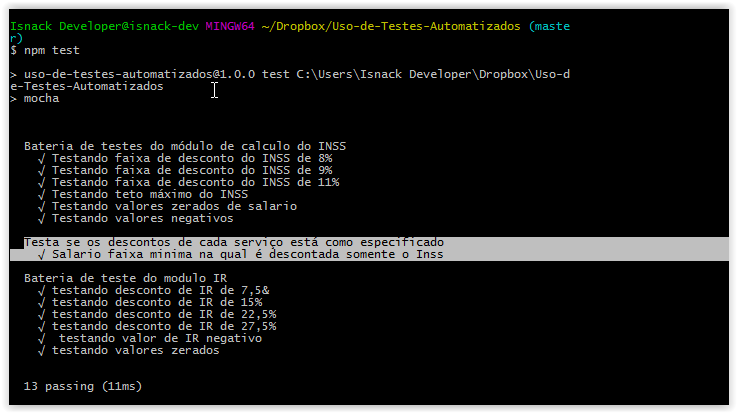
\includegraphics[scale=0.5]{imagens/teste22.png}
   
     \textbf{Fonte: } Elaborado pelos autores.}
     \label{fig:teste de integração sendo rodado novamente}
\end{figure}


\par Passando o primeiro teste foram criados outros testes para verificar se a integração entre as unidades de cálculo de desconto do INSS e do Imposto de Renda estavam corretas.


  \par As condições usadas para fazer os outros testes:
\begin{enumerate}

 \item Verificar se colocar um salário que não possua desconto do Imposto de Renda, com isso foi possível verificar se o módulo de Imposto de Renda poderia afetar o cálculo do salário líquido. Conforme mostra o Código 12.
 
  \item Fazer a verificação se o módulo realizou o desconto de 9\% do INSS e de 7,5\% do Imposto de Renda.
  \item Fazer a verificação se o módulo realizou o desconto de 11\% do INSS e 15\% do Imposto de Renda.
  \item Fazer a verificação se o módulo realizou o desconto de 11\% do INSS e 22,5\% do Imposto de Renda.
  \item Fazer a verificação se o módulo realizou o desconto do teto \end{enumerate}
  
\newpage
 
\begin{lstlisting} [language=JavaScript, caption={[ Todos os testes do salário líquido.]{ Todos os testes do salário líquido.  \textbf{Fonte:} Elaborado pelos autores.}}]
var expect = require('chai').expect;
var salarioLiquidoService = require('../app/services/SalarioLiquidoService');

describe('Testa se os desconto de cada servico está como especificado',function(){
    
it('Faixa minima na qual é descontada somente o Inss',function(){
  expect(salarioLiquidoService.calculate(1500)).to.equal(1380);
});
it('Faixa 9% de desconto do Inss com desconto de IR faixa de 7.5%',function(){
  expect(salarioLiquidoService.calculate(2300)).to.be.closeTo(2078.83,0.01);
});
it('Faixa 11% de desconto do Inss com desconto de IR faixa de 15%',function(){
  expect(salarioLiquidoService.calculate(3200)).to.be.closeTo(2775.60,0.01);
});
it('Faixa 11% de desconto do Inss com desconto de IR faixa de 22,5%',function(){
   expect(salarioLiquidoService.calculate(4450.00)).to.be.closeTo(3705.52,0.01);
});
it('Desconto teto do Inss com desconto de IR faixa de 27,5%',function(){
 expect(salarioLiquidoService.calculate(5200.00)).to.be.closeTo(4223.70,0.01)
});    
});    
    
    
\end{lstlisting}
\begin{comment}
\begin{figure}[!htb]
     \caption[Todos os Teste do salário liquido ]{Todos os Teste do salário liquido.
     \centering
     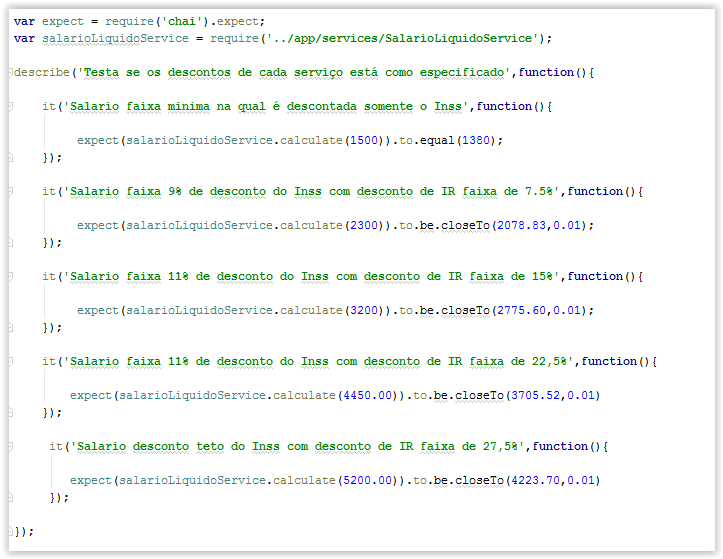
\includegraphics[width=12cm,height=6cm]{imagens/teste23.png}
     
     \textbf{Fonte: } Elaborado pelos autores.}
     \label{fig:todos os Teste do salário liquido}
\end{figure}
\end{comment}

\par Nesse teste foi utilizado a função de comparação de resultados \texttt{to.be.closeTo}, nessa função é informado o valor que se deseja comparar com um intervalo de tolerância no resultado, que no caso é de 0.01.

\par Com os testes de unidade e integração prontos, a próxima etapa foi a realização dos testes funcionais. Foi necessário a criação do modelo de banco de dados utilizando o \textit{MongoDB} e a configuração dos serviços em \textit{RestApi} e depois a criação das páginas \textit{web}.

\newpage
\par Primeiramente foi criado a estrutura para guardar os dados no \textit{MongoDB} e, portanto foi utilizado o \textit{mongoose} para criar essa estrutura, conforme mostra o Código 13.



\begin{lstlisting}[language=JavaScript, caption={[Estrutura Documento MongoDB.]{Estrutura Documento MongoDB.  \textbf{Fonte:} Elaborado pelos autores.}}]
var mongoose = require('mongoose');
var funcionarioSchema = new mongoose.Schema({
  nome: String,
  endereco: String,
  cidade: String,
  estado: String,
  bairro: String,
  salario:Number
 });

\end{lstlisting}

\par Com essa estrutura é possível guardar os seguintes dados:
 \begin{itemize}
  \item Nome;
  \item Endereço;
  \item Cidade;
  \item Estado;
  \item Bairro;
   \item Salário.
 \end{itemize}

\par Para o servidor \textit{Rest} foi utilizado o \textit{framework Restify} com as seguintes rotas:
\begin{itemize}
 \item \textbf{Contexto da aplicação:} \url{http://<endereço_servidor/<rota>};
 
 \item \textbf{api/funcionarios:} obter lista de funcionários via \textit{get};
 
\item \textbf{api/folhaSal/:id:} Obter folha salarial por id do funcionário via \textit{get};

\item \textbf{api/funcionarios/:id:} obter funcionário específico por id via \textit{get};

\item \textbf{api/funcionários:}  Enviar registro de funcionários via \textit{post};

\item \textbf{api/funcionarios:} Atualizar registro de funcionário via \textit{put};

\item \textbf{api/funcionarios/:id:} Deletar funcionário via \textit{delete};

\item \textbf{api/authentication:} Realizar autenticação de usuário via \textit{post}.

\end{itemize}

\par Para a criação das páginas foi utilizado o \textit{Bootstrap} e o \textit{AngularJS} e atribuiu-se as seguintes responsabilidades:
\begin{itemize}
 \item Autenticar;
 \item Listar Funcionários;
 \item Adicionar Funcionário;
 \item Gerar Folha de Pagamento.
\end{itemize}

\par As páginas utilizam esses serviços que foram citados anteriormente, com tudo isso pronto inicia-se a criação dos testes funcionais.

\par Para a criação dos testes funcionais foi utilizado o \textit{framework CasperJS}, o qual já foi demonstrada sua instalação anteriormente.


\par Primeiramente é criado o arquivo de teste na pasta \texttt{test}, mas ao rodar os testes unitários o \textit{mocha} acabava rodando os testes do \textit{CasperJS}, pois o \textit{mocha} não é preparado para rodar o \textit{CasperJS}, para resolver esse problema foi necessário criar uma pasta somente para os testes funcionais.

\par Criado um roteiro para testar toda a aplicação, na qual consiste em simular o usuário acessando o sistema, fazendo o login
com dados incorretos e depois com dados corretos, verificando se o sistema dá o retorno para o usuário de que algo está errado ou ocorreu algum problema.

\par Depois de verificar se a página que ele está dando acesso é a correta, no qual deverá aparecer a lista de funcionários, depois adicionar um novo funcionário, gerar folha de pagamento do mesmo, podendo atualizar esse cadastro e por último fazer sua exclusão. Com esse roteiro é iniciado a criação do \textit{script} que executam os testes


\par Dentro do projeto foi criado uma pasta denominada \texttt{testFunctional}, e dentro dessa pasta foi criado o arquivo \texttt{functionalTest.js}. Foi necessário criar uma função \texttt{casper.test\\.begin} para iniciar os testes, essa função tem como parâmetros o nome da bateria de testes e a quantidade de testes que serão realizados.

\par Para começar o teste precisa realizar a autenticação, para isso foi criado um método para realizar esse procedimento, no Código 14, como pode ser observado, primeiro é feito a chamada do método do objeto formulário \texttt{testAutenticacao}, e passado a instância do \textit{CasperJS} que é a variável \texttt{casper}, esse método tem como responsabilidade realizar o teste de autenticação de usuário.

\newpage
\begin{lstlisting}[language=JavaScript, caption={[Chamada da função para o teste de autenticação.]{Chamada da função para o teste de autenticação. \textbf{Fonte:} Elaborado pelos autores.}}]
casper.test.begin('Teste Funcional da Folha de Pagamento', 15, function (test) {
       formulario.testAutenticacao(casper);
}

\end{lstlisting}

\par No Código 15 primeiro é chamado o método \texttt{casper.start} que é responsável em acessar a aplicação \textit{web}, informando uma url na qual a aplicação está sendo executada.



\begin{lstlisting}[language=JavaScript, caption={[Acessar aplicação utilizando método casper.start.]{Acessar aplicação utilizando método casper.start.  \textbf{Fonte:} Elaborado pelos autores.}}]
testAutenticacao:function(casper){
        casper.start('http://localhost:8585/public/');
            casper.then(function (casper) {
                this.test.assertExists(x('//*[@id="botao"]'), 'Testando se existe o botão de login');
        });
            casper.then(function () {
                 this.click(x('//*[@id="botao"]'));
         });
}
\end{lstlisting}

\par O método \texttt{test.assertExists} testa se existe um elemento que é especificado, e a variável \texttt{x} é uma instância para o \textit{CasperJS} entender o \textit{XPath} e sua instanciação é feita no começo do \textit{script}, como demonstra o Código 16.


\begin{lstlisting}[language=JavaScript, caption={[Atribuição para o seletor de XPath.]{Atribuição para o seletor de XPath.  \textbf{Fonte:} Elaborado pelos autores.}}]
var x = require('casper').selectXPath;

\end{lstlisting}


\par Feito essa instanciação, o teste é capaz de selecionar elementos via \textit{XPath} para selecionar o elemento utilizando \textit{XPath} basta carregar a página desejada, apertar o botão F12 do teclado, selecionar a aba \textit{elements}, clicar com o botão direito em cima do elemento e depois selecionar a opção \textit{copy} e em seguinda \textit{copy XPath}, conforme mostra a Figura 17, esse processo é feito em todos os elementos necessários para realização do teste.


\newpage

\begin{figure}[!htb]

     \caption[Copiar o XPath ]{Copiar o XPath.
     
     \raggedleft
      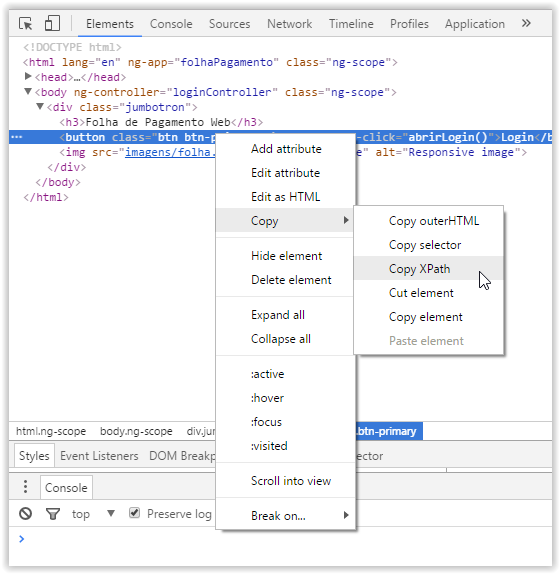
\includegraphics[width=15cm,height=20cm]{imagens/teste51.PNG}
   \centering
     \textbf{Fonte: } Elaborado pelos autores.}
     \label{fig:Copiar o XPath}
\end{figure}

\newpage

\par Com o \textit{XPath} selecionado o método \texttt{test.assertExists} verifica se existe o elemento com a identificação \texttt{*[@id="botao"]}.

\par Os procedimentos do teste ficam dentro do método \texttt{casper.then}, esse método adiciona um passo que o \textit{script} deve fazer, então é chamado o método \texttt{click} e nesse método é informado o \textit{XPath} do botão de \textit{login}, assim, possibilita o acesso à página de login, como pode ser observado no Código 15.

\par Na página de \textit{login} é necessário informar usuário e senha, para o \textit{script} fazer isso é necessário chamar o método \texttt{sendKeys} e informar o elemento que é desejado e no outro parâmetro a informação, que nesse caso o usuário é "admin".


\begin{lstlisting}[language=JavaScript, caption={[Teste que verifica a validação da página.]{Teste que verifica a validação da página. \textbf{Fonte:} Elaborado pelos autores.}}]
casper.then(function () {
    this.sendKeys('#usuario', 'admin');
});
casper.then(function () {
    this.capture('testFunctional/img/teste3.png');
});
casper.then(function () {
    this.test.assertTextExists('Por favor, preencha os campos!', 'Testando se no corpo da pagina contém a frase "Por favor, preencha os campos!"');
});
\end{lstlisting}

\par Segundo o teste, informar somente o \textit{login} e verificar se a página exibe a informação "Por favor, preencha os campos!", esse teste está verificando a validação do formulário e se está funcionando corretamente. Para realizar o teste é chamando o método \texttt{test.assertTextExists} e a sua função é testar se o texto "Por favor, preencha os campos!" foi exibido na página ou se está no corpo da página como exemplifica o Código 17.

\par Para auxiliar na produção do teste a função \texttt{capture} auxilia a fazer um \textit{debug} no teste, possibilitando assim, visualizar após a execução do teste como a página estava no momento que foi executado o procedimento.


\par Depois foi informado a senha errada, o \textit{script} clica no botão enviar utilizando o método \texttt{click} passando o \textit{XPath} especificado no botão.

\newpage

\begin{lstlisting}[language=JavaScript, caption={[Teste que verifica a validação da página novamente.]{Teste que verifica a validação da página novamente.  \textbf{Fonte:} Elaborado pelos autores.}}]
casper.then(function () {
    this.sendKeys('#senha', 'admin1');
    this.click(x('//*[@id="loginForm"]/div[5]/div/button'));
});
casper.wait(3000, function () {
    this.echo("Esperando Resposta do Servidor!!");
});
casper.then(function () {
    this.test.assertTextExists('Usuario e/ou senha inválidos','Testando se o usuário foi impedido de entrar e se a mensagem de alerta é a correta"');
});

\end{lstlisting}

\par O teste verifica se a informação "Usuario e/ou senha inválidos" foi exibido, utilizando o método \texttt{test.assertTextExists}, no qual testa a condição do Código 18. Outra função importante é o \texttt{wait}, nela tem a possibilidade de colocar um tempo de espera em milissegundos no teste que será executado, pois em vários casos a página que está sendo testada carrega em menor velocidade que o processamento do teste, sendo necessário utilizar essa função.


\begin{lstlisting}[language=JavaScript, caption={[Teste que verifica o título da página.]{Teste que verifica o título da página.  \textbf{Fonte:} Elaborado pelos autores.}}]
casper.then(function () {
  this.test.assertTitle("Funcionários", "Testando se está na página de Funcionários");      
});

\end{lstlisting}

\par No ultimo teste são informados os dados corretos e é testado se o título da página é "Funcionários". Para realizar esse teste foi utilizado o método \texttt{test.assertTitle} informando o título desejado. Com isso se compara o título processado na página, como exemplifica o Código 19.

\par Outro teste realizado neste trabalho foi a verificação do conteúdo da página de gerar folha de pagamento, para esse propósito foi criado o método \texttt{testGerarFolhaSalarial} do objeto formulário.

\newpage


\begin{lstlisting}[language=JavaScript, caption={[Teste que verifica a folha de pagamento.]{Teste que verifica a folha de pagamento.  \textbf{Fonte:} Elaborado pelos autores.}}]
casper.wait(3000, function () {
  this.echo("Esperando Pagina Carregar Proxima página!!");
});
casper.then(function () {
  this.test.assertExists(x("/html/body/table/tbody/tr[3]/td[5][normalize-space()='"+descontoIr+"']"),'Testando o valor de desconto do IR está impresso');
});
casper.then(function () {
 this.capture('img/teste55.png');
  this.test.assertExists(x("/html/body/table/tbody/tr[4]/td[5][normalize-space()='"+descontoInss+"']"),'Testando o valor de desconto do IR está impresso');
});
casper.then(function(){
  this.test.assertExists(x("/html/body/table/tbody/tr[2]/td[4][normalize-space()='"+salario+"']"),'Testando o valor salario está impresso');           
});
casper.then(function(){
  this.test.assertExists(x("/html/body/table/tbody/tr[7]/td[5][normalize-space()='"+salarioLiquido+"']"),'Testando o valor salario Líquido está impresso');           
});
casper.then(function () {
  this.test.assertExists(x("/html/body/table/thead/tr/th [normalize-space()='Nome: "+nome+"']"),'Testando se o nome do funcionário está impresso');
});
casper.waitForSelector(x('/html/body/input'), function () {
  this.click(x('/html/body/input'));
});
casper.wait(3000, function () {
  this.echo("Esperando Pagina Carregar Proxima página!!");
});
}

\end{lstlisting}

\par No Código 20 a função recebe uma instância do \textit{CasperJS}, os valores esperados do desconto do INSS e IR, o salário bruto e líquido além do nome do funcionário.

\newpage

\par O teste consiste em verificar se o elemento no qual é impresso a informação é o esperado, como pode ser observado na linha 5 do Código 20, a função utilizada foi \texttt{assertExists}, no qual testa se o elemento informado, que no caso é \textit{XPath}, existe a diferença é que tem a função \texttt{normaliza-space}, que retorna uma \textit{string} sem espaços, sendo assim essa função retorna verdadeiro quando encontra o desconto do IR no elemento informado no teste.


\par Com todas as etapas criadas, a execução do teste é iniciada com o comando \textit{"casperjs test testFunctional/functionalTest.js"}. 

\begin{figure}[!htb]

     \caption[Log dos testes executados com sucesso]{Log dos testes executados com sucesso.
    \centering
      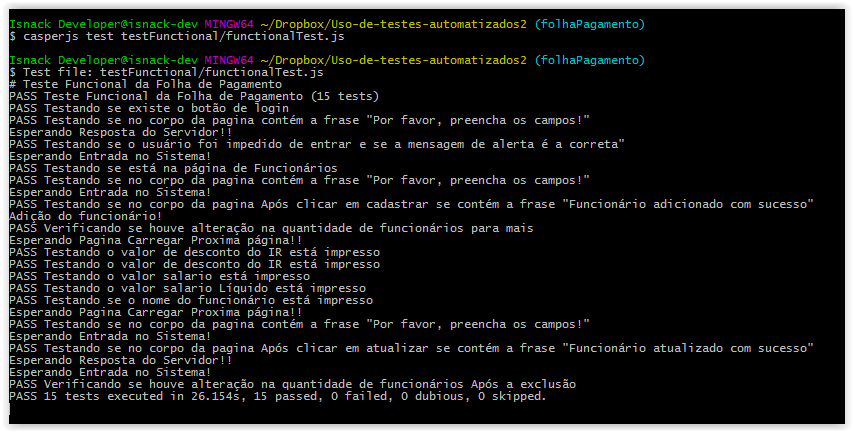
\includegraphics[width=13cm,height=13cm]{imagens/teste34.PNG}
   
     \textbf{Fonte: } Elaborado pelos autores.}
     \label{fig:Log dos testes executados com sucesso}
\end{figure}

\par A Figura 18 mostra o \textit{log} dos testes executados com sucesso, como pode-se reparar, no final é mostrado o tempo de execução de 26 segundos, mostrando assim, que os testes funcionais demoram um tempo maior para finalizar se comparados aos testes de unidade.

\par Na Figura 19 mostra-se um caso em que ocorreu um erro na execução do teste, ele mostra que o elemento especificado não foi encontrado, nesse caso há possibilidade do teste ter sido executado sem esperar a página carregar totalmente. Para fazer o teste passar é só colocar um tempo de esperar utilizando a função \texttt{wait}, como foi explicado durante os testes.


\begin{figure}[!htb]

     \caption[Teste mostrando erro]{Teste mostrando erro.
    \centering
      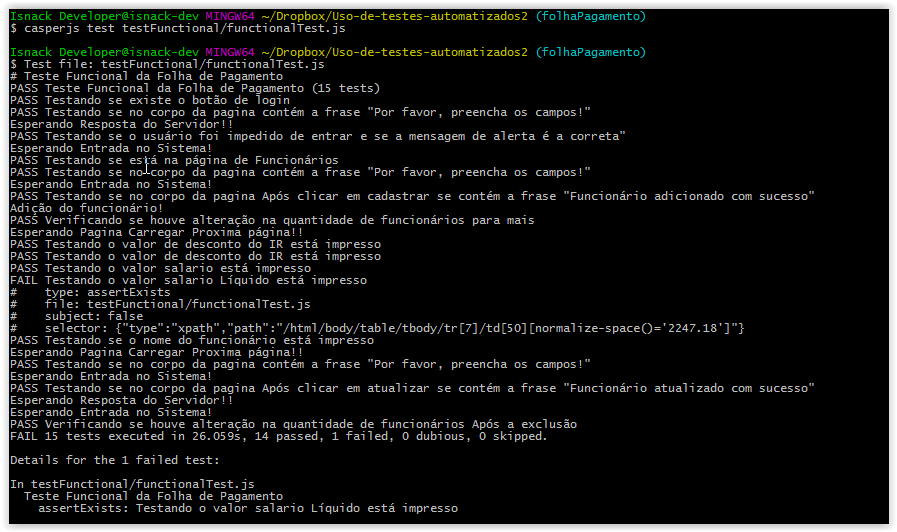
\includegraphics[width=13cm,height=13cm]{imagens/teste35.PNG}
   
     \textbf{Fonte: } Elaborado pelos autores.}
     \label{fig:Teste mostrando erro}
\end{figure}


\par O tempo de execução dos testes funcionais foi em média 26 segundos, se comparado com os testes de unidade e bem mais demorado.



\newpage
\section{TravisCI}

\par Para poder utilizar integração contínua, foi necessário configurar uma conta no \textit{TravisCI}.
 \par Primeiramente é feito a criação de um arquivo na raiz do projeto nomeado \texttt{travis.yml} esse arquivo será responsável pela configuração da \textit{build}. A Figura 20 é o exemplo de configuração.

\begin{figure}[!htb]

     \caption[Configuração inicial do TravisCI ]{Configuração inicial do TravisCI.
     \centering
      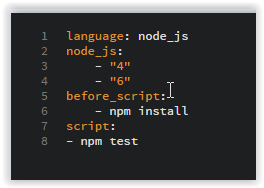
\includegraphics[width=12cm,height=6cm]{imagens/travis1.png}
   
     \textbf{Fonte: } Elaborado pelos autores.}
     \label{fig:configuração inicial do TravisCI}
\end{figure}


\begin{itemize}
 
 \item \textit{Language} é a definição da linguagem a ser usada na hora de criar a \textit{build} do projeto.
 
 \item \textit{Before script} é uma seção para especificar um comando antes de executar o \textit{script} principal, no projeto é executado para instalar todas as dependências que estão listadas no \texttt{package.json}.
 
 \item \textit{Script} é o lugar que será executado algum comando para execução dos testes e integração da solução. 
 
\end{itemize}

\par Após a criação do arquivo \texttt{travis.yml} é necessário dar permissão para o serviço \textit{TravisCI} acessar os repositórios da conta do \textit{GitHub}, e só utilizar a opção \textit{login} pelo \textit{GitHub} que automaticamente é pedido as permissões de acesso, então aceitá-las.
\par Com as permissões aceitas, é só adicionar o repositório desejado no \textit{TravisCI}, a Figura 20 demonstra essa ilustração.
 \newpage
\begin{figure}[!htb]
     \caption[Adicionar repositório no TravisCI ]{Adicionar repositório no TravisCI.
     \centering
     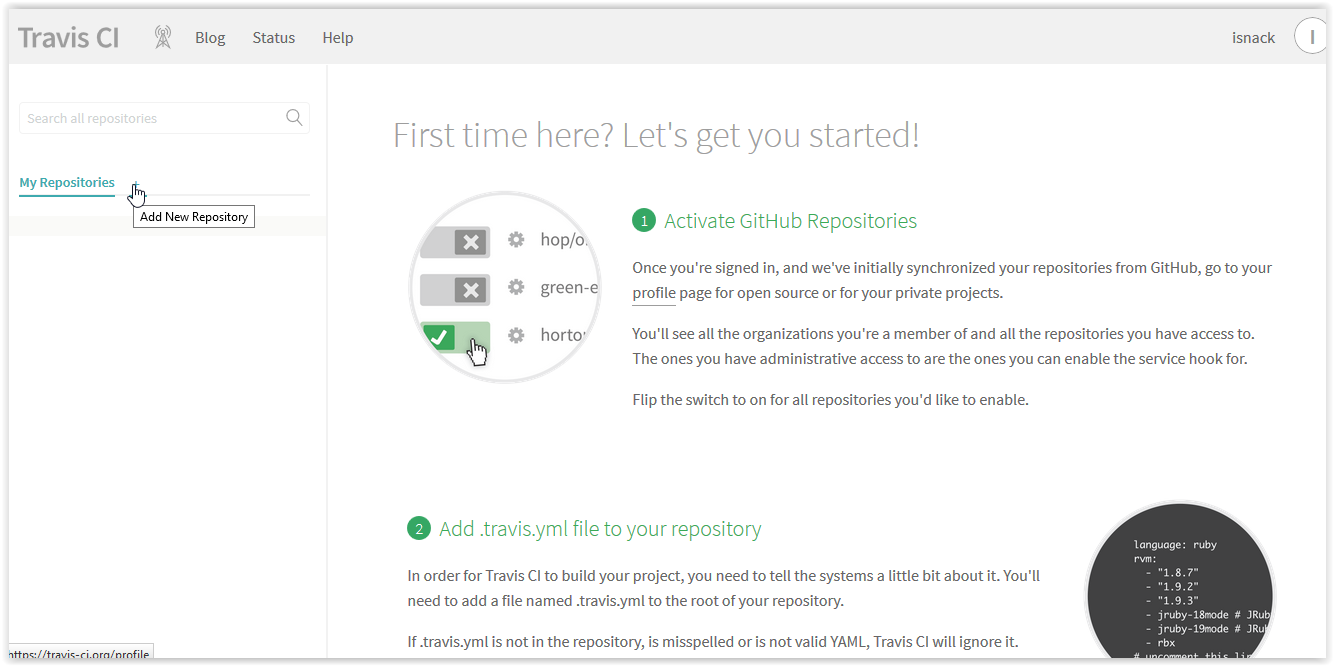
\includegraphics[width=12cm,height=6cm]{imagens/travis2.png}
    
     \textbf{Fonte: } Elaborado pelos autores.}
     \label{fig:adicionar repositório no TravisCI}
\end{figure}
 
 

\par Acessar \textit{Add New Repository} \footnote{Adicionar novo repositório}, caso seja a primeira vez que está acessando o \textit{TravisCI} é necessária uma sincronização com sua conta do \textit{GitHub}. A Figura 21 faz essa demonstração.

\begin{figure}[!htb]
    \caption[Sincronização do TravisCI com GitHub ]{Sincronização do TravisCI com GitHub.
     \centering
     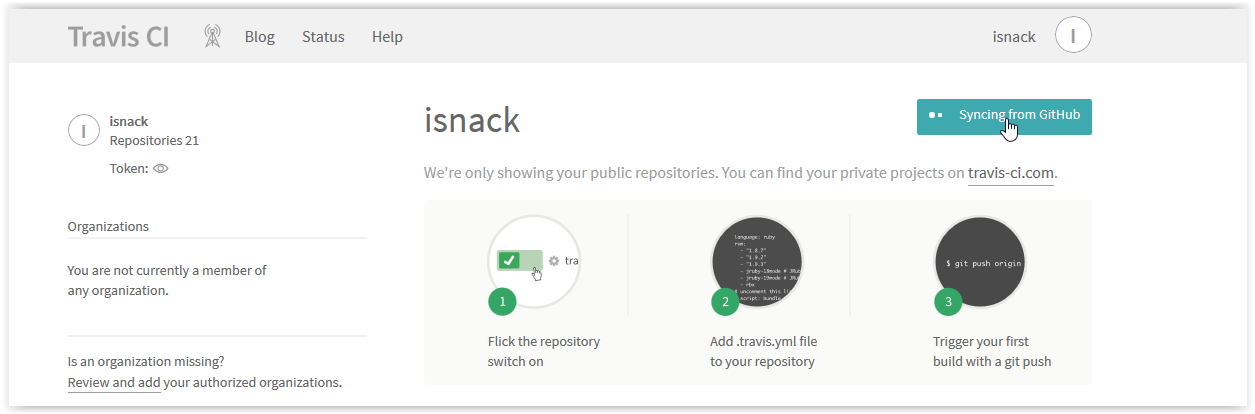
\includegraphics[width=12cm,height=6cm]{imagens/travis3.png}
     
     \textbf{Fonte: } Elaborado pelos autores.}
     \label{fig:sincronização do TravisCI com GitHub}
\end{figure}

\par Feita a sincronização da conta do \textit{GitHub} são listados todos os repositórios, selecionar o repositório em que serão feitos os testes, e feita a configuração, conforme mostra Figura 22.

\newpage
\begin{figure}[!htb]
    
    \caption[Repositório em que é feito a configuração do TravisCI  ]{Repositório em que é feito a configuração do TravisCI.
     \centering
     
\includegraphics[width=15cm,height=3cm]{imagens/travis4.png}
     
     \textbf{Fonte: } Elaborado pelos autores.}
     \label{fig:repositório em que é feito a configuração do TravisCI}
\end{figure}


\par Após a ação acima são apresentadas algumas configurações, conforme mostra Figura 24.

\begin{figure}[!htb]
    \caption[Configurações do TravisCI ]{Configurações do TravisCI.
     \centering
     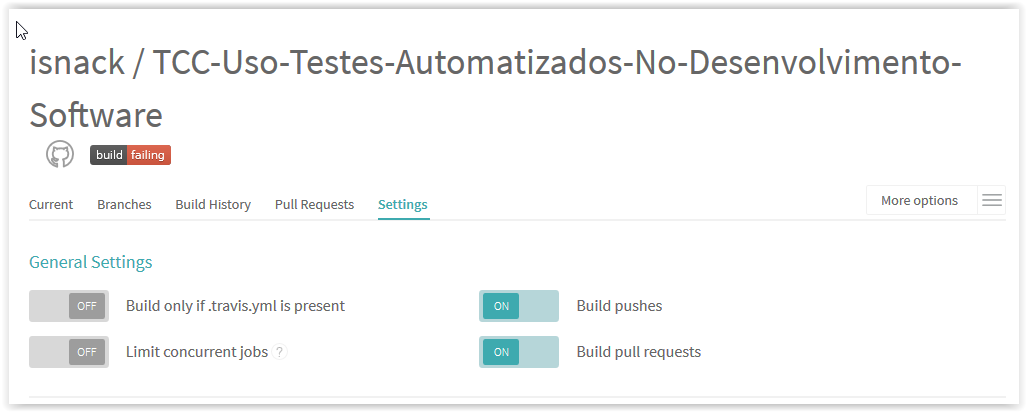
\includegraphics[width=12cm,height=6cm]{imagens/travis5.png}
     
     \textbf{Fonte: } Elaborado pelos autores.}
     \label{fig:configurações do TravisCI}
\end{figure}

\begin{itemize}
 
\item \textit{Build Pushes} é todo \textit{commit} ou alteração no código do repositório, o \textit{TravisCI} executará novamente a \textit{build}, executando todos os testes programados.

\item \textit{Build Only IF .travis.yml} o \textit{travisCI}, só irá executar uma integração se o arquivo de configuração estiver presente no repositório.
 
 \item \textit{Build pull requests}, é executado uma integração toda vez que tiver um \textit{pull request}
 
 \item \textit{Build History} é o local de armazenamento dos \textit{log} de todas as \textit{builds} executadas durante a criação do projeto.
 
\end{itemize}


\par Feito as configurações no repositório o \textit{Travis} está habilitado para testar a aplicação conforme mostra Figura 25.
\newpage
\begin{figure}[!htb]
    \caption[TravisCI está pronto para realização dos testes ]{TravisCI está pronto para realização dos testes.
     \centering
     
\includegraphics[width=15cm,height=3cm]{imagens/travis6.png}
      \textbf{Fonte: } Elaborado pelos autores.}
     \label{fig:TravisCI está pronto para realização dos testes}
\end{figure}

\par O primeiro \textit{commit} que foi feito no projeto, o \textit{travis} criará uma máquina virtual rodando o S.O \footnote{Sistema Operacional} Ubuntu, conforme mostra Figura 26.


\begin{figure}[!htb]
     \caption[TravisCI recebendo os commits ]{TravisCI recebendo os commits.
     \centering
     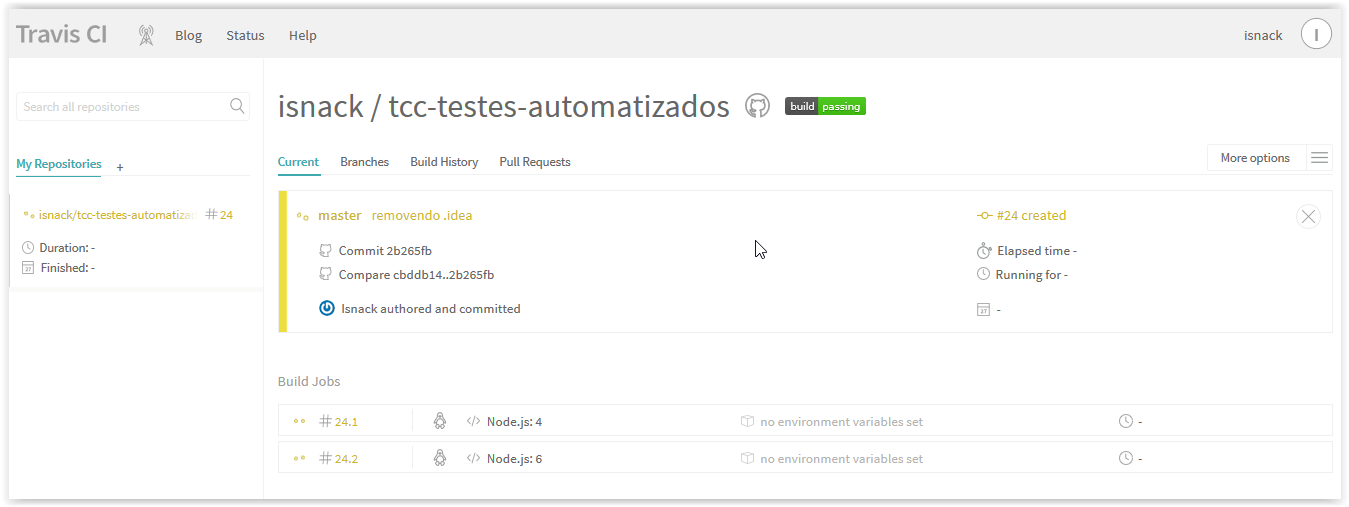
\includegraphics[width=15cm,height=9cm]{imagens/travis7.png}
      \textbf{Fonte: } Elaborado pelos autores.}
     \label{fig:travisCI recebendo os commits}
\end{figure}
 
 \par O projeto está sendo construído no repositório e sua cor fica em amarelo, para fazer essa referência, o \textit{Build Jobs} são as versões de linguagem, sinalizando que o seu projeto está sendo integrado e testado.

\par Na Figura 27 é mostrado o \textit{log} de inicialização do projeto, e pode se ver detalhes de como está sendo executado o projeto em si.
\newpage
\begin{figure}[!htb]
     \caption[Log de Inicialização ]{Log de Inicialização.
     
     \raggedleft
     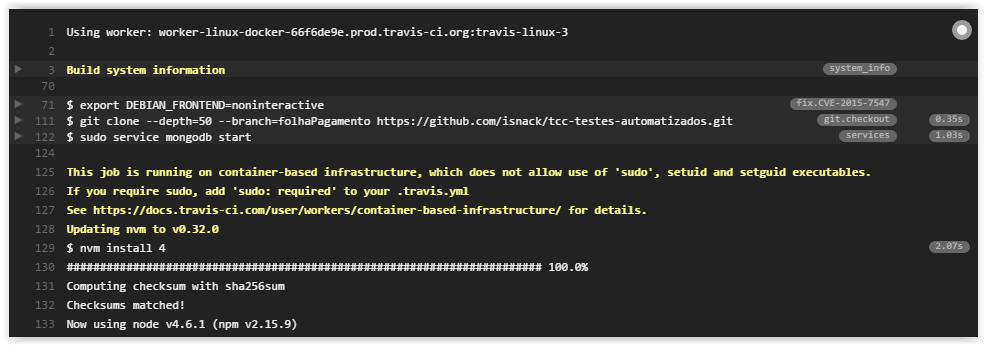
\includegraphics[scale=.60]{imagens/travis8.png}
     \centering
     \textbf{Fonte: } Elaborado pelos autores.}
     \label{fig:log de Inicialização}
\end{figure}


\par Após a execução do projeto, caso os testes falhem, o \textit{log} é responsável por mostrar para o desenvolvedor em qual linha ocorreu o erro, conforme mostra Figura 28.

\begin{figure}[!htb]
\centering
    \caption[Log mostrando o erro ]{Log mostrando o erro.
     
     
     \centering
     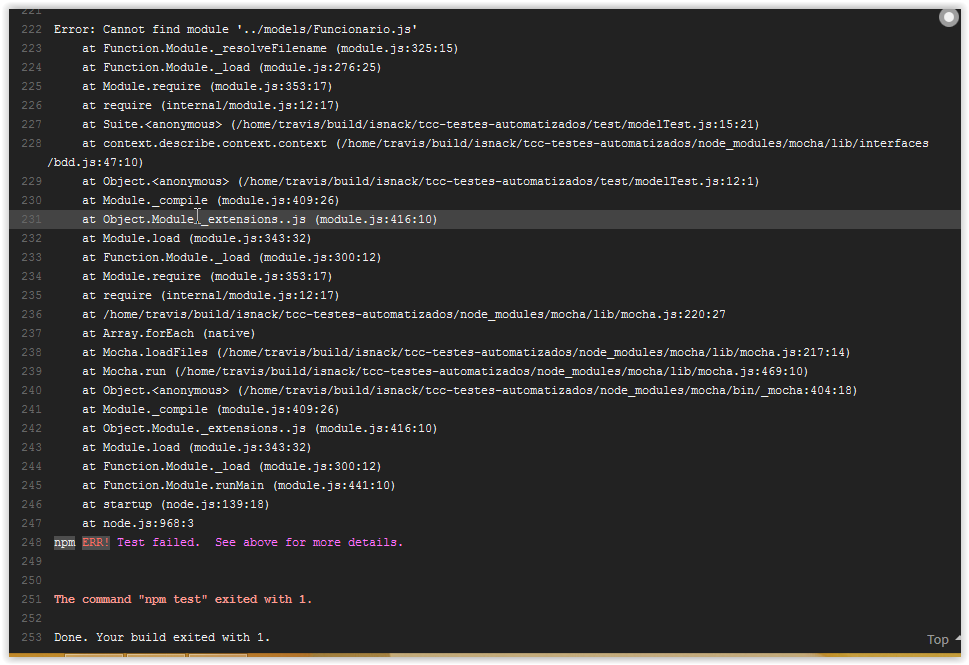
\includegraphics[width=15cm,height=9cm]{imagens/travis9.png}
     
     \centering
      \textbf{Fonte: } Elaborado pelos autores.}
     \label{fig:log mostrando o erro}
\end{figure}


\par Observando a Figura 28, o erro mostrado é o módulo do banco chamando o funcionário não encontrado, com esse \textit{feedback}, é necessário corrigir a chamada do módulo, para que seja executado com sucesso o teste. Caso os testes passem, é apresentado no painel a cor verde, indicando que os testes foram executados com sucesso. A Figura 29 mostra o \textit{log} no qual os testes passaram.

\newpage
\begin{figure}[!htb]
    \caption[Log com sucesso ]{Log com sucesso.
     
      \raggedleft
     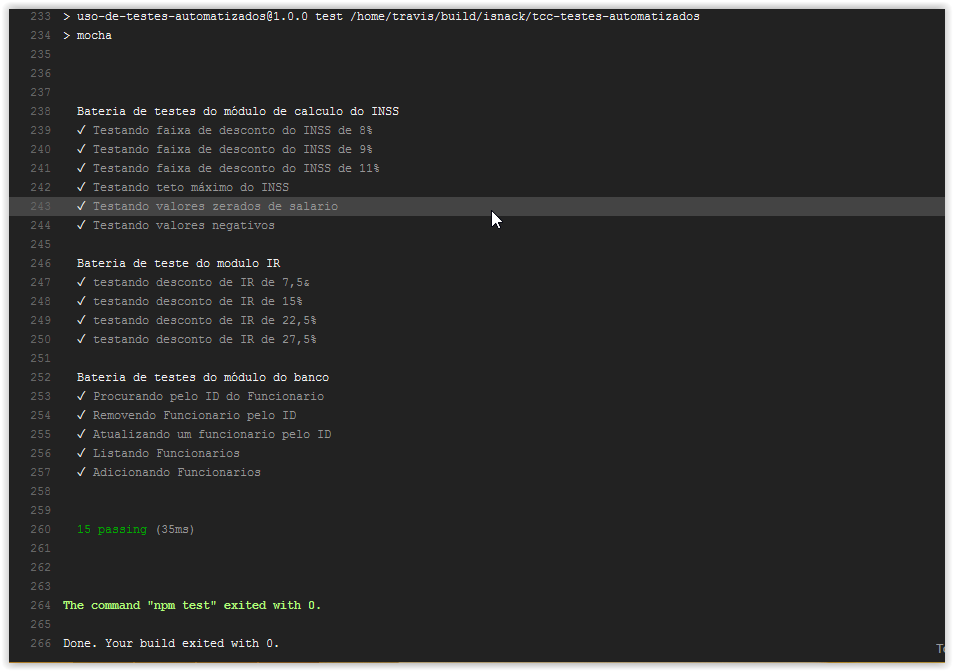
\includegraphics[width=15cm,height=9cm]{imagens/travis10.png}
     
     \centering
     \textbf{Fonte: } Elaborado pelos autores.}
     \label{fig:log com sucesso}
\end{figure}

\par O \textit{TravisCI} disponibiliza o histórico de tudo que foi feito no decorrer do projeto.
\par Essa funcionalidade ajuda muito o desenvolvedor a verificar como foi o andamento do projeto, e se houveram muitos erros que foram vistos e corrigidos no decorrer do desenvolvimento, a Figura 30 explica isso.

\begin{figure}[!htb]
    \caption[Históricos dos commits no TravisCI ]{Históricos dos commits no TravisCI.
     
     \raggedleft
     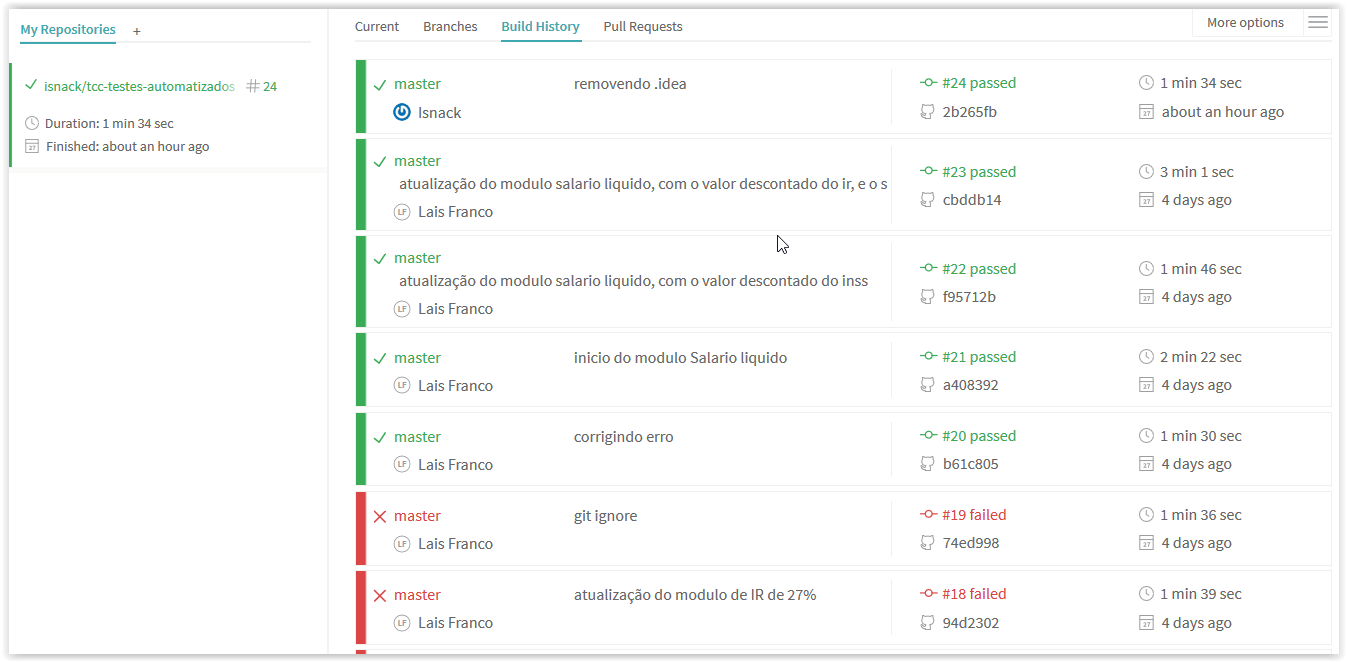
\includegraphics[width=15cm,height=9cm]{imagens/travis11.png}
     
     \centering
     \textbf{Fonte: } Elaborado pelos autores.}
     \label{fig:históricos dos commits no TravisCI}
\end{figure}

\newpage
\par Houve duas integrações que quebraram, e o autor corrigiu o erro, e novamente enviou com as alterações feitas, para que o projeto voltasse a funcionar normalmente. Durante esse processo todos os membros da equipe ficam a par do que está acontecendo, e se o responsável enviar uma \textit{build} quebrada outro membro da equipe pode resolver o problema.

\par O \textit{TravisCI} disponibiliza outro meio de ver os \textit{logs} de execução com ou sem sucesso.

\par Através do \textit{e-mail}, toda vez que um teste é executado os membros da equipe recebem um \textit{e-mail} mostrando se aquela versão está quebrada ou não, conforme mostra Figura 31.
 
\begin{figure}[!htb]
    \caption[E-mail que o TravisCI envia ]{E-mail que o TravisCI envia.
     \centering
     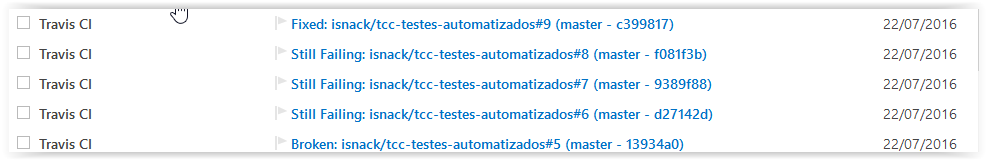
\includegraphics[width=14cm,height=3cm]{imagens/travis12.png}
     \textbf{Fonte: } Elaborado pelos autores.}
     \label{fig:e-mail que o TravisCI envia}
\end{figure}


\par Ao abrir a mensagem se vê mais detalhes e o link para o \textit{TravisCI}, e visualizar com detalhes o \textit{log} de inicialização, execução dos testes e o link para comparação do código antigo e o novo.



\par Outra funcionalidade é a integração contínua, quando se tem um \textit{pull request}, o \textit{TravisCI} executa a integração quando se tem uma nova contribuição no repositório. Conforme mostra a Figura 32, o \textit{TravisCI} executa a integração  quando se tem um \textit{pull request}.


\begin{figure}[!htb]
    \caption[Pull Request no TravisCi ]{Pull Request no TravisCi.
     \centering
     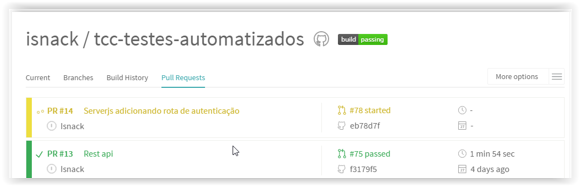
\includegraphics[width=12cm,height=6cm]{imagens/travis13.PNG}
     
     \textbf{Fonte: } Elaborado pelos autores.}
     \label{fig:Pull Request no TravisCi}
\end{figure}

\newpage
\par Assim o gerente ou o responsável pelo repositório não tem a necessidade de baixar a requisição e testar em uma máquina, o \textit{TravisCI} se encarrega dessa tarefa, desta forma, poupa-se tempo.

\par A Figura 33 apresenta um \textit{checklist} mostrando se a integração contínua está sem quebrar, desse jeito o botão de \textit{merge} no \textit{GitHub} fica verde, para efetuar o procedimento de junção do código.

\begin{figure}[!htb]
    \caption[Checklist ]{Checklist.
    
     \centering
     \includegraphics[width=12cm,height=6cm]{imagens/travis14.PNG}
     
     \textbf{Fonte: } Elaborado pelos autores.}
     \label{fig:Checklist}
\end{figure}


\par Caso contrário o \textit{checklist} fica com os itens em vermelho, indicando que teve falha na integração, conforme mostra a Figura 34.

\newpage
\begin{figure}[!htb]
    \caption[Checklist mostrando erro ]{Checklist mostrando erro.
    
     \centering
     \includegraphics[width=12cm,height=6cm]{imagens/travis15.PNG}
     
     \textbf{Fonte: } Elaborado pelos autores.}
     \label{fig:Checklist mostrando erro}
\end{figure}

\par Todos esses eventos são notificados por \textit{email}, assim toda equipe fica por dentro das integrações feitas no repositório.

\newpage
\section{Relatório de Cobertura}


\par Nessa seção é demonstrada a configuração do relatório de cobertura de testes para geração localmente e a utilização do serviço \texttt{coveralls.io}, esse relatório é necessário para obter a informação de como os testes criados no projeto estão cobrindo as unidades criadas.

\par Para isso primeiramente foi configurado o relatório localmente para esse propósito  é necessário instalar um pacote no NPM chamado \textit{istanbul}, com o seguinte comando \texttt{npm install istanbul –g}, esse pacote é rapidamente instalado.

\par Após esse procedimento, é necessário configurar na seção de \textit{scripts} do NPM, como mostra a Código 21.



\begin{lstlisting}[language=JavaScript, caption={[Configurar o relatório de cobertura com o NPM.]{Configurar o relatório de cobertura com o NPM.  \textbf{Fonte:} Elaborado pelos autores.}}]
"scripts":{
"test": "mocha",
"coveralls-local" : "istanbul cover ./node_modules/mocha/bin/_mocha"

},
\end{lstlisting}

\begin{comment}
\begin{figure}[!htb]
    \caption[Configurar o relatório de cobertura com o NPM  ]{Configurar o relatório de cobertura com o NPM.
    
     \centering
     \includegraphics[width=15cm,height=4cm]{imagens/relatorio.PNG}
     
     \textbf{Fonte: } Elaborado pelos autores.}
     \label{fig:Configurar o relatório de cobertura com o NPM}
\end{figure}
\end{comment}

\par Adicionando o comando coveralls-local: “istanbul cover ./node\_modules/mocha/Bin/\\\_mocha”, após realizar a configuração, foi executado comando npm run coveralls-local, deste modo foi criado uma pasta chamada \texttt{coverage} dentro do projeto e nela são criados arquivos em HTML os quais contém os relatórios de cobertura. A Figura 35 ilustra os arquivos contidos na pasta \texttt{coverage}.



\begin{figure}[!htb]
    \caption[Criado pasta coverage ]{Criado pasta coverage.
    
     \centering
     \includegraphics[width=15cm,height=4cm]{imagens/relatorio2.PNG}
     
     \textbf{Fonte: } Elaborado pelos autores.}
     \label{fig: Criado pasta coverage}
\end{figure}


\newpage

\par Ao abrir a pasta \texttt{lcov-report}, contém um arquivo chamado \texttt{index.html} e ao executar o mesmo, será apresentado o relatório de cobertura, como pode ser observado na Figura 36 o relatório separa por pasta.

\begin{figure}[!htb]
    \caption[lcov-report ]{ lcov-report.
    
     \centering
     \includegraphics[width=15cm,height=4cm]{imagens/relatorio3.PNG}
     
     \textbf{Fonte: } Elaborado pelos autores.}
     \label{fig:lcov-report}
\end{figure}

\par Dentro da pasta \texttt{services} contém todas unidades ou arquivos que contém lógica e nas quais os testes foram executados, o relatório exibe algumas informações como:

\begin{itemize}
 \item \textit{Statements}: Porcentagem de cobertura dos testes, ou seja, quantos por cento do código testado está sendo coberto pelo teste;
 \item \textit{Branches}: Cobertura nos \textit{Branches};
 \item \textit{Functions}: Cobertura nas funções;
 \item \textit{Lines}: Cobertura de linhas no código.
 
\end{itemize}

\begin{figure}[!htb]
    \caption[Relatório de Cobertura ]{Relatório de Cobertura.
    
     \centering
     \includegraphics[width=15cm,height=4cm]{imagens/relatorio4.PNG}
     
     \textbf{Fonte: } Elaborado pelos autores.}
     \label{fig:Relatório de Cobertura}
\end{figure}

\par A Figura 37 mostra que o código está com mais de 85\% coberto pelos testes, além do arquivo que está com o menor índice de cobertura, que nesse caso é de mais de 52\%, enquanto os outros arquivos estão com 100\% de cobertura.

\par Abrindo uma unidade com 100\% de cobertura e outra com 52\%, observa-se algumas informações.

\newpage
\begin{figure}[!htb]
    \caption[Relatório de Cobertura no qual  está 52\% coberto ]{Relatório de Cobertura no qual  está 52\% coberto.
    
     \centering
     \includegraphics[width=15cm,height=15cm]{imagens/relatorio5.PNG}
     
     \textbf{Fonte: } Elaborado pelos autores.}
     \label{fig:Relatório de Cobertura no qual não está 52\% coberto}
\end{figure}

\par A Figura 38 mostra quais as linhas estão necessitando que faça-se um teste, e essas linhas ficam destacadas em vermelho para facilitar a sua visualização.
\par A Figura 39 mostra um código que está com 100\% de cobertura, por isso fica tudo verde.

\newpage

\begin{figure}[!htb]
    \caption[Relatório de Cobertura no qual  está 100\% coberto ]{Relatório de Cobertura no qual  está 100\% coberto.
    
     \centering
     \includegraphics[width=12cm,height=10cm]{imagens/relatorio6.PNG}
     
     \textbf{Fonte: } Elaborado pelos autores.}
     \label{fig:Relatório de Cobertura no qual não está 100\% coberto}
\end{figure}

\par O relatório de cobertura demonstra que o projeto necessita de mais testes, e assim,  auxiliando no desenvolvimento dos testes no sistema que está sendo desenvolvido.

\par Feito a configuração da cobertura de testes localmente, também foi configurado \textit{online} utilizando o site \url{http://www.coveralls.io}.

\par O procedimento é a criação de uma conta no site citado acima, pode se utilizar a integração com \textit{GitHub} para criação da conta, sendo possível fazer a sincronização dos repositórios do \textit{GitHub}.

\begin{figure}[!htb]
    \caption[Sincronizando Github com o coveralls ]{Sincronizando Github com o coveralls.
    
     \centering
     \includegraphics[width=8cm,height=5cm]{imagens/relatorio7.PNG}
     
     \textbf{Fonte: } Elaborado pelos autores.}
     \label{fig:Sincronizando Github com o coveralls}
\end{figure}

\newpage

\par Feito a criação da conta no site, no menu do lado esquerdo  tem a opção \textit{add repositoy} (conforme mostra Figura 40), após esse procedimento  são listados todos os repositórios do \textit{GitHub}, depois é só habilitar o repositório da aplicação. Conforme mostra a Figura 41.

\begin{figure}[!htb]
    \caption[Listas de repositórios no GitHub ]{Listas de repositórios no GitHub.
    
     \centering
     \includegraphics[width=15cm,height=4cm]{imagens/relatorio9.PNG}
     
     \textbf{Fonte: } Elaborado pelos autores.}
     \label{fig:Listas de repositórios no GitHub}
\end{figure}

\begin{figure}[!htb]
    \caption[O setup do relatório de cobertura utilizando o TravisCI ]{O setup do relatório de cobertura utilizando o TravisCI.
    
     \centering
     \includegraphics[width=12cm,height=8cm]{imagens/relatorio8.PNG}
     
     \textbf{Fonte: } Elaborado pelos autores.}
     \label{fig:O setup do relatório de cobertura utilizando o TravisCI}
\end{figure}

\par Após a habilitação do repositório, a Figura 42 mostra como realizar o \textit{setup} do relatório de cobertura utilizado o serviço de integração contínua (\textit{TravisCI}). Com esses dados foi necessário criar o arquivo \texttt{.coveralls.yml}, nesse arquivo contém o parâmetro \texttt{repo\_token} que é um numero de identificação do repositório no site do \textit{coverlls}.
\par A Figura 43 demonstra a criação do arquivo \texttt{.coveralls.yml}, na pasta raiz do projeto e na Figura 44 o conteúdo do arquivo. 

\newpage

\begin{figure}[!htb]
    \caption[Criação do .coveralls.yml ]{Criação do .coveralls.yml.
    
     \centering
     \includegraphics[scale=1]{imagens/relatorio10.PNG}
     
     \textbf{Fonte: } Elaborado pelos autores.}
     \label{fig:Criação do .coveralls.yml}
\end{figure}

\begin{figure}[!htb]
    \caption[Rebo Token ]{Repo Token.
    
     \centering
     \includegraphics[scale=1]{imagens/relatorio11.PNG}
     
     \textbf{Fonte: } Elaborado pelos autores.}
     \label{fig:Rebo Token}
\end{figure}

\par Após esses procedimentos, foi necessária a instalação de um pacote, o \textit{coveralls} utilizando o npm , o comando \texttt{npm install coveralls  -- save} e depois a configuração do \textit{script} dentro do arquivo \texttt{package.json}.




\begin{lstlisting}[language=JavaScript, caption={[Configuração do script dentro do package.json.]{Configuração do script dentro do package.json.  \textbf{Fonte:} Elaborado pelos autores.}}]
"scripts": {
  "test": "mocha",
  "coveralls-local": "istanbul cover ./node_modules/mocha/bin/_mocha",
  "coveralls": "istanbul cover ./node_modules/mocha/bin/_mocha --report lcovonlu -- -R spec && cat ./coverage/lcov.info | ./node_modules/coveralls/bin/coveralls.js && rm -rd ./coverage"
 } 


\end{lstlisting}

\begin{comment}


\begin{figure}[!htb]
    \caption[Configuração do script dentro do package.json ]{Configuração do script dentro do package.json.
    
     \centering
     \includegraphics[width=16cm,height=4cm]{imagens/relatorio12.PNG}
     
     \textbf{Fonte: } Elaborado pelos autores.}
     \label{fig:Configuração do script dentro do package.json}
\end{figure}
\end{comment}

\par O Código 22 mostra a criação do \textit{script} chamado \textit{coveralls}, no qual o comando utilizado é “istanbul cover ./node\_modules/mocha/bin/\_mocha --report lcovonly -- -R spec \&\& cat ./coverage/lcov.info |   ./node\_modules/coveralls/bin/coveralls.js && rm -rf ./coverage”.


\par Esse \textit{script} roda o teste, cria o relatório de cobertura localmente e lê o arquivo \texttt{lcov.info}, no qual contém as informações de cobertura do teste e envia essas informações para o arquivo \texttt{coveralls.js}, que por sua vez, envia todas essas informações para o site do \textit{coveralls.io}.

\par Foi necessário adicionar mais uma linha de comando no arquivo \texttt{.travis.yml} que é o responsável pela integração com \textit{TravisCI}, foi adicionada a instalação do \textit{istanbul} no setor  \textit{before\_script}, no setor \textit{after\_script} e adicionado o \textit{script}  \texttt{npm run coveralls}, que será executado logo após o \textit{script} principal de integração. Conforme mostra Figura 45.

\begin{figure}[!htb]
    \caption[Adicionando linhas de comando no .travis.yml ]{Adicionando linhas de comando no .travis.yml.
    
     \centering
     \includegraphics[width=16cm,height=9cm]{imagens/relatorio13.PNG}
     
     \textbf{Fonte: } Elaborado pelos autores.}
     \label{fig:Adicionando linhas de comando no .travis.yml}
\end{figure}

\par Após realizar as configurações, deve-se fazer algum \textit{commit} ou \textit{pull request}, o relatório é gerado após a integração feita pelo \textit{TravisCI}. A Figura 46 demonstra um relatório gerado pelo site \url{www.coveralls.io}.


\begin{figure}[!htb]
    \caption[Relatório gerado pelo coveralls.io ]{Relatório gerado pelo coveralls.io.
    
     \centering
     \includegraphics[width=15cm,height=8cm]{imagens/relatorio14.PNG}
     
     \textbf{Fonte: } Elaborado pelos autores.}
     \label{fig:Relatório gerado pelo coveralls.io}
\end{figure}

\newpage
\par O relatório demonstra as mesmas informações do que é gerado localmente como: cobertura do arquivo, linhas, quais dessas linhas são relevantes e as linhas de maior relevância estão cobertas.

\par Um exemplo interessante ao se criar um \textit{pull request} é a integração do \textit{coveralls.io} com \textit{GitHub}, o site notifica a porcentagem de cobertura e se a cobertura se manteve ou se caiu comparando com o código atual. A Figura 47 faz essa demonstração.

\begin{figure}[!htb]
    \caption[Notificação de porcentagem de cobertura ]{Notificação de porcentagem de cobertura.
    
     \centering
     \includegraphics[width=15cm,height=9cm]{imagens/relatorio15.PNG}
     
     \textbf{Fonte: } Elaborado pelos autores.}
     \label{fig:Notificação de porcentagem de cobertura}
\end{figure}


\par Nesse caso, a cobertura dos testes era de 100\% e teve uma redução de mais de 14\%, essa informação é de grande relevância, pois a partir dela decide-se quando aceitar o \textit{pull request}  e se o responsável pelo projeto requer uma porcentagem específica de cobertura dos testes ou não.

\par No \textit{coveralls.io} é possível criar uma configuração, que caso o \textit{pull request} tiver uma cobertura menor que 90\% seja considerado como falha, ou então se a cobertura cair uma porcentagem específica também é considerado como falha. Para esse propósito basta acessar o repositório que está com relatório de cobertura e clicar no link \textit{Settings} como mostra a Figura 48.

\newpage
\begin{figure}[!htb]
    \caption[Configuração do coveralls.io ]{Configuração do coveralls.io.
    
     \centering
     \includegraphics[width=12cm,height=7cm]{imagens/relatorio16.PNG}
     
     \textbf{Fonte: } Elaborado pelos autores.}
     \label{fig:Configuração do coveralls.io}
\end{figure}

\par A opção \textit{Coverage threshold for failure} é opção de alerta quando a cobertura cair abaixo de 90\% como ilustra a Figura 48. E a opção \textit{Coverage decrease threshold for failure} alerta quando a cobertura cair uma porcentagem que pode ser especificada, Ex: mais de 15\% será emitido um alerta.

\par A Figura 49 mostra um \textit{branch} que não está de acordo com as regras especificadas, ficando assim marcado com um “x” em vermelho indicando que não está de acordo.

\begin{figure}[!htb]
    \caption[Branch que não está de acordo com as regras especificadas ]{Branch que não está de acordo com as regras especificadas.
    
     \centering
     \includegraphics[scale=0.60]{imagens/relatorio17.PNG}
     
     \textbf{Fonte: } Elaborado pelos autores.}
     \label{fig:Branch que não está de acordo com as regras especificadas}
\end{figure}
\begin{comment}


\newpage
\section{Participantes}

\par Isnack e Laís foram os responsáveis pelo planejamento, execução e testes do \textit{software} e também análise e desenvolvimento da pesquisa e suas conclusões.

\par Isnack Souza Novais, Técnico em informática formado pelo INPETTECC, possui experiência em desenvolvimento com linguagem de programação ".NET" e manipulação de banco de dados SQL SERVER, cursando o 8º período do Curso de Sistemas de Informação
da Universidade do Vale do Sapucaí.

\par Laís Vidal de Oliveira, cursando 8º período do curso de Sistemas de Informação da Universidade do Vale do Sapucaí e fazendo curso de Testes Automatizados e C\#. 

\par Ednardo David Segura – Pós-graduado em Engenharia Web pela Universidade Federal de Itajubá – UNIFEI (2008). Possui graduação em Ciência da Computação pelo Centro de Ensino Superior em Gestão, Tecnologia e Educação – FAI (2006). Atualmente é Especialista em Sistemas Sênior do Inatel Competence Center e Professor em cursos de Pós-Graduação no INATEL e da graduação na Univás. Possui experiência em desenvolvimento de software nas linguagens JavaScript (client/server), Java SE/EE, PHP, Groovy, para a plataforma web atuando principalmente nos seguintes temas: Telecomunicações, IPTV/OTT e Cloud Computing. Possui bons conhecimentos em programação orientada a objetos, programação funcional e desenvolvimento orientado a testes.

\end{comment}


\clearpage
\newpage

\begin{comment}

\section{Cronograma}

\par Abaixo descrito no cronograma as ações a serem seguidas no projeto, desde a definição até a conclusão.

\begin{figure}[!htb]
     \centering
 \includegraphics[width=17cm,height=17cm]{imagens/cronograma6.png}
     \caption[Cronograma do desenvolvimento do projeto]{Cronograma do desenvolvimento do projeto.
     \textbf{Fonte: } Elaborado pelos autores.}
     \label{fig:cronograma}
\end{figure}

\clearpage
\newpage

\section{Orçamento}
\par Abaixo o orçamento com as despesas detalhadas previstas para a realização do projeto.

\begin{figure}[!htb]
     \centering
     \includegraphics[width=17cm,height=17cm]{imagens/orcamento.png}
     \caption[Orçamento previsto do projeto]{Orçamento previsto do projeto.
     \textbf{Fonte: } Elaborado pelos autores.}
     \label{fig:orcamento}
\end{figure}


\end{comment}










\begin{comment}
Exemplo de código Java:

\begin{lstlisting} [style=custom_Java,caption={[Métodos da classe \texttt{FilmeBean}]{Métodos da classe \texttt{FilmeBean}. \textbf{Fonte:} Elaborado pelos autores.}}, label=fig:metodosclassebean] 	
	public FilmeBean(){  
       //...
   	}	
   	
	public void saveMovie(){
		setListActorSelected();		
		if(this.movieDAO.saveMovieGraph(this.movieTo)){
			FacesContext.getCurrentInstance().addMessage(null, 
			   new FacesMessage("Filme cadastrado com sucesso!")); 
		}else{
			//...
		}		
		this.limpaCampos();
	}
\end{lstlisting}

\par Agora será mostrado o exemplo do uso de fluxo de eventos apresentado no Quadro~\ref{quad:fluxo_evento_cadastro_filme}.

\begin{quadro}[h!]
  \begin{fluxoDeEventos}
  \addTitle{Cadastrar filme}
  \addrow{Ator principal}{Administrador}
  %\addrow{Ator secundário}{Sistema de cartão}
  \addrow{Pré-requisitos}{Estar logado no sistema}

  \startBasicFlow{Ator} {Sistema}
  \addItemOne{Seleciona menu cadastro}
  \addItemOne{Clica na opção cadastrar filme}
  \addItemTwo{Abre interface de cadastro de filme}
  \addItemOne{Preenche formulário}
  \addItemOne{Clica no botão salvar}
  \addItemTwo{Salva e informa sucesso no cadastro}

  \startAlternativeFlow{Fluxo alternativo 1}
  \addItemOne{No item 5, formulário não preenchido}
  \addItemTwo{Exibe mensagem de necessidade de preenchimento de formulário}

  \startAlternativeFlow{Fluxo alternativo 2}
  \addItemOne{No item 6, inserido filme já cadastrado}
  \addItemTwo{Informa mensagem de filme já cadastrado}
\end{fluxoDeEventos}

  \caption[Fluxo de eventos para cadastro de filme]
           {Fluxo de eventos para cadastro de filme. \textbf{Fonte:} Elaborado pelos autores}
  \label{quad:fluxo_evento_cadastro_filme}
\end{quadro}

\par Outro exemplo é ilustrado na Figura~\ref{fig:bluesky}. Neste caso um código XML foi embutido dentro de um ambiente de figura, para que este código seja incluído no índice de figuras adequadamente.
 
\begin{figure}[ht!]
  \begin{lstlisting} [style=custom_XML]
	...
	<context-param>
		<param-name>primefaces.THEME<\param-name>
		<param-value>bluesky<\param-value>
	<\context-param>
	...
  \end{lstlisting}
 
  \caption[Incluindo o tema \textit{BlueSky} ao contexto do projeto]
          {Incluíndo o tema \textit{BlueSky} ao contexto do projeto. \textbf{Fonte:} Elaborado pelos autores.}
  \label{fig:bluesky}
\end{figure}
\end{comment}